
% \documentclass{article} % For LaTeX2e
% \usepackage{icml2025,times}

% % Optional math commands from https://github.com/goodfeli/dlbook_notation.
% \input{math_commands.tex}

% \usepackage{hyperref}
% \usepackage{url}
% \usepackage{subcaption}
% \usepackage{graphicx}
% \usepackage{amsthm}
% \usepackage{ulem}
% \usepackage{algorithm} % For the floating algorithm environment
% \usepackage{algorithmicx} % For the floating algorithm environment

% % \usepackage{algpseudocode} % For algorithmic pseudocode commands

% \newcommand{\theHalgorithm}{\arabic{algorithm}}


% % \usepackage{natbib}
% % \usepackage{subfigure}

% \title{Conformal Decision Theory for AI Agents}

% \author{
%     Drew Prinster \& Kyunghyun Cho \& Clara Fannjiang \& Samuel Stanton \\
%     Genentech \\
%     1 DNA Way, San Francisco, CA \\
%     \texttt{\{prinster.drew,stanton.samuel\}@gene.com}
% }

\newcommand{\fix}{\marginpar{FIX}}
\newcommand{\new}{\marginpar{NEW}}
\newcommand{\drew}[1]{\textcolor{blue}{[Dr: #1]}}



% % \iclrfinalcopy % Uncomment for camera-ready version, but NOT for submission.
% \begin{document}


% \maketitle

%%%%%%%% ICML 2025 EXAMPLE LATEX SUBMISSION FILE %%%%%%%%%%%%%%%%%

\documentclass{article}

% Recommended, but optional, packages for figures and better typesetting:
\usepackage{microtype}
\usepackage{graphicx}
\usepackage{subfig}
\usepackage{subcaption}
\usepackage{booktabs} % for professional tables
\usepackage{bbm}

\usepackage{tikz}

\usepackage{xcolor}

\usepackage{hyperref}
\usepackage{url}
\usepackage{subcaption}
% \usepackage{graphicx}
\usepackage{amsthm}
\usepackage{ulem}

% hyperref makes hyperlinks in the resulting PDF.
% If your build breaks (sometimes temporarily if a hyperlink spans a page)
% please comment out the following usepackage line and replace
% \usepackage{icml2025} with \usepackage[nohyperref]{icml2025} above.
\usepackage{hyperref}


% Attempt to make hyperref and algorithmic work together better:
\newcommand{\theHalgorithm}{\arabic{algorithm}}

% Use the following line for the initial blind version submitted for review:
\usepackage[preprint]{icml2025}

% If accepted, instead use the following line for the camera-ready submission:
% \usepackage[accepted]{icml2025}

% For theorems and such
\usepackage{amsmath}
\usepackage{amssymb}
\usepackage{mathtools}
\usepackage{amsthm}


\usepackage{pifont}% http://ctan.org/pkg/pifont

\newcommand{\cmark}{\Large\textcolor{green!80!black}{\ding{51}}}
\newcommand{\xmark}{\Large\textcolor{red}{\ding{55}}}
% \usepackage{fourier}
\newcommand{\mygreen}[1]{{\color{green!60!black}#1}}


% if you use cleveref..
\usepackage[capitalize,noabbrev]{cleveref}

%%%%%%%%%%%%%%%%%%%%%%%%%%%%%%%%
% THEOREMS
%%%%%%%%%%%%%%%%%%%%%%%%%%%%%%%%
\theoremstyle{plain}
\newtheorem{theorem}{Theorem}[section]
\newtheorem{proposition}[theorem]{Proposition}
\newtheorem{lemma}[theorem]{Lemma}
\newtheorem{corollary}[theorem]{Corollary}
\theoremstyle{definition}
\newtheorem{definition}[theorem]{Definition}
\newtheorem{assumption}[theorem]{Assumption}
\theoremstyle{remark}
\newtheorem{remark}[theorem]{Remark}

% Todonotes is useful during development; simply uncomment the next line
%    and comment out the line below the next line to turn off comments
%\usepackage[disable,textsize=tiny]{todonotes}
\usepackage[textsize=tiny]{todonotes}

\DeclareMathOperator*{\argmax}{arg\,max}
\DeclareMathOperator*{\argmin}{arg\,min}

% The \icmltitle you define below is probably too long as a header.
% Therefore, a short form for the running title is supplied here:
\icmltitlerunning{Conformal Policy Control}

\begin{document}

\twocolumn[
\icmltitle{Conformal Policy Control}

% It is OKAY to include author information, even for blind
% submissions: the style file will automatically remove it for you
% unless you've provided the [accepted] option to the icml2025
% package.

% List of affiliations: The first argument should be a (short)
% identifier you will use later to specify author affiliations
% Academic affiliations should list Department, University, City, Region, Country
% Industry affiliations should list Company, City, Region, Country

% You can specify symbols, otherwise they are numbered in order.
% Ideally, you should not use this facility. Affiliations will be numbered
% in order of appearance and this is the preferred way.
\icmlsetsymbol{equal}{*}

\begin{icmlauthorlist}
\icmlauthor{Drew Prinster}{gen,jhu}
\icmlauthor{Clara Fannjiang}{gen}
\icmlauthor{Ji Won Park}{gen}
\icmlauthor{Kyunghyun Cho}{gen}
\icmlauthor{Samuel Stanton}{prev_gen}
% \icmlauthor{Firstname5 Lastname5}{yyy}
% \icmlauthor{Firstname6 Lastname6}{sch,yyy,comp}
% \icmlauthor{Firstname7 Lastname7}{comp}
% %\icmlauthor{}{sch}
% \icmlauthor{Firstname8 Lastname8}{sch}
% \icmlauthor{Firstname8 Lastname8}{yyy,comp}
%\icmlauthor{}{sch}
%\icmlauthor{}{sch}
\end{icmlauthorlist}

\icmlaffiliation{gen}{Prescient Design,
Genentech, U.S.A.}
\icmlaffiliation{jhu}{Johns Hopkins University}
\icmlaffiliation{prev_gen}{Formerly Prescient Design, Genentech}

\icmlcorrespondingauthor{Drew Prinster}{drewprinster@gmail.com}
\icmlcorrespondingauthor{Samuel Stanton}{sdstanton1@gmail.com}

% You may provide any keywords that you
% find helpful for describing your paper; these are used to populate
% the "keywords" metadata in the PDF but will not be shown in the document
\icmlkeywords{Machine Learning, ICML}

\vskip 0.3in
]

% this must go after the closing bracket ] following \twocolumn[ ...

% This command actually creates the footnote in the first column
% listing the affiliations and the copyright notice.
% The command takes one argument, which is text to display at the start of the footnote.
% The \icmlEqualContribution command is standard text for equal contribution.
% Remove it (just {}) if you do not need this facility.

\printAffiliationsAndNotice{}  % leave blank if no need to mention equal contribution
% \printAffiliationsAndNotice{\icmlEqualContribution} % otherwise use the standard text.


\begin{abstract}
\drew{Note: This was a placeholder abstract, will revise}
Enabling AI agents to automate or inform high-stakes decision-making inevitably involves risks, but it is often precisely in real-world, high-stakes settings where those risks are most difficult to control or quantify. Prime examples include iterative biomolecular design and active learning, where an AI system that chooses where to query its next data point induces dependencies between successive data distributions that can cause standard uncertainty- and risk-quantification methods to lose validity. This paper develops Conformal Decision Theory for AI Agents: a practical and statistically principled methodological framework for enabling black-box AI agents to automatically determine their own ``zone of competence'' based on their training data, in order to design experiments with guarantees on the hit rate (or other user-specified criteria of interest) over time. Underlying this framework is our algorithm for ``conformal policy control,'' which generalizes prior methods for conformal risk control to both non-exchangeable data distributions and to broader risk functions. We demonstrate the utility of our methods on real-world datasets. 
\end{abstract}


\section{Introduction}


Consequential decision making often requires navigating a fundamental tension between probable safety on the one hand, and a chance of extraordinary success  on the other. This dilemma has many variations and is known by many names, such as the explore-exploit trade-off in reinforcement learning, the strategies of diversification versus specialization in long-term planning, and the tenets of safety versus efficacy in clinical trials. In statistics, even the tradeoff between validity (i.e., controlling false discoveries or ``Type I'' errors) versus power or efficiency (i.e., maximizing the true detection rate or controlling ``Type II'' errors) has a similar flavor. More broadly, the ongoing debate as to how to balance ensuring AI systems are safe, versus advancing their capabilities to benefit society, urgently demands progress toward principled and practical solutions. 


This tension between AI safety and capabilities becomes even more prominent and challenging as these systems are increasingly endowed with \textit{agency}---the ability to act autonomously, with consequences to human well-being often at stake. In particular, deploying AI agents at scale poses at least three fundamental challenges: (1) Firstly, agents' actions over time may create what we refer to as \textit{feedback-loop shifts}---successive data distributions that are dependent on previous distributions---which can invalidate standard statistical inference.
% (which is often premised on a ``static world'' assumption of distributional invariance). 
Prime examples include experimental design, where an agent's decision about what experiment to run changes the distribution where it receives feedback, and robotics, where an agent chooses new physical environments to explore. (2) Secondly, generative AI agents based on large language models (LLMs) have large, potentially infinite action spaces. For instance, in biomolecular engineering, this might be the space of all possible protein sequences, while for LLM chatbots, it could be the space of possible text responses or chain-of-thought sequences. (3) Lastly, it is important to ensure that any risks being managed align with the values of the human stakeholders. For instance, there has been surging progress in uncertainty and risk \textit{quantification} of AI outputs in recent years, but a question largely remains: how can this methodological progress be translated in real-world practice, to \textit{improve decision making and outcomes}?


% (Decision making, dilemma of safety versus uncertainty)

% (Challenges with AI agents: Feedback loop shifts, large action spaces, risk criteria of interest to human end users)

% (Conformal prediction and conformal risk control)


    
    \begin{table*}[ht]
    \caption{Summary comparison of selected related work on conformal prediction for decision making under agent-induced shifts.}
    \centering
    {\small
    \begin{tabular}{ c | c | c | c  c  c } 
    \toprule
    % \cline{3-4}
    & & &  \multicolumn{3}{|c}{\textbf{3. Type of Risk Control}}  \\ 
     % \cmidrule(lr){2-4}
     % \multirow{2}{*}{2} & Rep-tile: & $\set{2}$ & $\set{3}$ & \\
     % \cline{2-4}
     % &  &  &  &  &  \\
     %%
      $\begin{matrix}
      \textbf{Method Group}\\ 
      \text{References}
      \end{matrix}$ & $\begin{matrix}
        \textbf{1. Agent-} \\
            \textbf{Induced} \\
           \textbf{Data Shift}
       \end{matrix}$
     & $\begin{matrix}
     \textbf{2. Action} \\ 
     \textbf{Space}
     \end{matrix}$ & $\begin{matrix}\textbf{Prediction Set} \\ \textbf{Miscoverage} \\ \mathbbm{1}\{Y_t\not\in \hat{C}_{\color{blue}\alpha}(X_t)\} \end{matrix}$ & $\begin{matrix}\lambda\textbf{-Parameterized} \\ \textbf{Losses} \\ L_t(A_t({\color{blue}\lambda}))\end{matrix}$ & 
      $\begin{matrix}
          \textbf{Unparameterizable} \\
          \textbf{Losses} \\
          \textbf{($\beta$-Param. Policy)} \\
          L_t(A_t), \ A_t\sim p_t({\color{blue}\beta})
      \end{matrix}$
       \\
     \hline
     $\begin{matrix}\textbf{Conformal Prediction} \\ 
     \text{\citet{vovk2005algorithmic}}
     \\
     \text{\citet{vovk2018conformal}} 
     \end{matrix}$ & \xmark & $\begin{matrix}
         \text{Small/} \\ \text{Finite}
     \end{matrix}$ & \cmark & \xmark & \xmark \\
     \hline
     $\begin{matrix}\textbf{Weighted Conformal Pred.} \\ 
     \text{\citet{tibshirani2019conformal}}
     \\
     \text{\citet{fannjiang2022conformal}} \\
     \text{\citet{stanton2023bayesian}} \\
     \text{\citet{nair2023randomization}} \\
     \text{\citet{prinster2024conformal}} \\
     \end{matrix}$  & $\begin{matrix} 
         \text{Single-Round} \\ 
    
         \hline \\
         \textbf{\mygreen{Multi-Round}} 
     \end{matrix}$ & $\begin{matrix}
         \text{Small/} \\ \text{Finite} \\ \hline  \text{Contin.} \\ \hline \text{Small/} \\ \text{Finite}
     \end{matrix}$ & \cmark & \xmark & \xmark \\
     \hline
     $\begin{matrix}\textbf{Conformal Risk Control} \\ 
     \text{\citet{angelopoulos2022conformal}}
     \\
     \text{\citet{lekeufack2024conformal}} 
     \end{matrix}$ & $\begin{matrix}
      \\
         \text{Single-Round} \\ 
         \hline 
         \text{Eventually safe}
     \end{matrix}$ & $\begin{matrix}
         \text{Small/} \\ \text{Finite} 
     \end{matrix}$ & \cmark & \cmark & \xmark \\
     \hline
     $\begin{matrix} \textbf{Conformal Policy Control} \\
     \text{(Proposed)}
     \end{matrix}$ & \textbf{\mygreen{Multi-Round}} & $\begin{matrix}
         \text{Large/} \\ \boldsymbol{\infty}
     \end{matrix}$ & \cmark & \cmark & \cmark  \\
    \bottomrule 
    \end{tabular}
    }
    \label{table:comparisons}
    \end{table*}
    

While decision making under uncertainty has been widely studied across AI/ML, statistics, economics, and other fields, most existing reliability guarantees fail to hold in the case of AI agents. That is, most approaches to statistical uncertainty quantification---a prerequisite to statistical decision theory---rely on restrictive parametric assumptions (which are difficult to verify or enforce), require distributional invariance  (e.g., independent and identically distributed or ``IID'' data) which is violated by feedback-loop shifts, or only provide a weak form of ``long-run'' or ``eventual'' safety. A noteable exception is \textit{conformal prediction} (CP) \citep{vovk2005algorithmic, angelopoulos2024theoretical}, for which standard variants provide nonparametric guarantees \citep{vovk2005algorithmic} and recent ``weighted'' extensions have advanced the ability to handle certain agent-induced feedback-loop shifts \citep{tibshirani2019conformal, fannjiang2022conformal, nair2023randomization, prinster2024conformal}. 


In this work, we build on recent progress in conformal prediction to develop \textit{conformal policy control} (CPC): a practical and statistically-principled framework for enabling black-box AI agents to automatically determine their own ``zone of competence'' based on their available data, where they are able to respect a user-specified risk constraint. Our CPC methods can be viewed as extending conformal risk control (CRC) \citep{angelopoulos2022conformal} to enable controlling risks where one cannot directly parameterize the loss function (as is needed in CRC), but where one can control the \textit{probabilities} or \textit{policy} governing the risk. Our CPC methods address the key challenges posed by AI agents---that is, of feedback-loop shifts, large/infinite action spaces, and flexible, user-specified risk-criteria---and achieve \textit{nonparametric, test-time} reliability guarantees (Table \ref{table:comparisons}). We evaluate our proposed methods on real-world data with a simulated active learning task, as well as on a rigorous biomolecular design benchmark with LLM agents.





% \drew{(Placeholder intro)}

% A machine learning (ML) model is only as good as its data.
% All too often we set out to solve a problem with ML only to find the initial data we were given are insufficient for the task.
% As a result solving a problem with ML entails not only finding the right model, but also constructing the right dataset.
% When relevant data is easy to find constructing a dataset is primarily a matter of aggregation and curation.
% When relevant data is expensive to obtain it becomes a matter of \textit{exploration} and \textit{prioritization}.
% What data can we collect that makes the best use of the resources we have?

% Algorithmic solutions to efficient data collection go by various names depending on the exact problem setting (e.g. active learning, black-box optimization, reinforcement learning, etc.).
% Most of these algorithms iteratively construct a dataset by training a predictive model on the data already collected and then give the model \textit{agency} to decide which data to collect next.
% If all goes well, a virtuous cycle is created.
% When these algorithms are integrated into systems deployed to consequential settings, we quickly find we cannot allow them to operate unconstrained.
% To operate reliably, we need to control the risk the system incurs while it improves.

% Quantifying risk requires quantifying the uncertainty of our predictions.
% While there are many statistical approaches to uncertainty quantification, most rely on critical distributional assumptions that are difficult to verify or enforce, which limits their practical utility.
% Conformal prediction \citep{vovk2005algorithmic} is a notable exception, as it makes no assumptions about the exact form of the data distribution, but instead relies on more abstract assumptions like exchangeability.
% Unfortunately the data generated by AI agents is not exchangeable, since the data collected at each point in time are statistically dependent on the data that came before.

% \citet{fannjiang2022conformal} proved that conformal prediction could be extended to AI agents for a single round starting from an i.i.d. dataset, building on a key result from \citet{tibshirani2019conformal} for independently (but not identically) distributed data.
% In this work we show that \citet{tibshirani2019conformal}'s results can be reinterpreted to show that conformal prediction can in theory be extended to \textit{any} joint distribution (including ones with sequential dependencies), although the fully general form is not practically feasible ($\mathcal{O}((n+1)!)$) to compute.
% In particular we show that a conformal coverage guarantee for AI agents over multiple rounds is not only theoretically possible, but one of the special cases where the guarantee can be realized in practice.
% To support our theory we provide empirical results on synthetic protein design and active learning tasks which verify that we maintain coverage when baselines from \citet{tibshirani2019conformal} and \citet{fannjiang2022conformal} fail to do so.


\vspace{-0.25cm}

\section{Problem Setup and Background}



\subsection{General Setup: Risk-Constrained Decision Making}


At each time $t=0, 1, ...$, the agent receives an input context (or observation, state, or prompt) $X_t\in \mathcal{X}$ and takes an action $A_t\in\mathcal{A}$. For example, in the setting of LLMs, $X_t$ could be a text prompt, with $\mathcal{X}=\mathcal{V}^*$ for a vocabulary $\mathcal{V}$, and the LLM's action could be to generate a text response $A_t(X_t)=X_t'$. 
% , which can in turn produce some output $X_t'\in \mathcal{X}$. 
% which for now we will assume is a function on the input space, $A_t:\mathcal{X}\rightarrow \mathcal{X}$. 
After taking action, the agent receives some feedback (e.g., from a human or the environment) in the form of a response (or label) $Y_t'\in \mathcal{Y}$.\footnote{Here, we keep notation simple in two main ways: First, we initially assume a fully online setting, where feedback is received after every action; later we will introduce notation for a ``minibatch'' setting, where feedback may be received only intermittently after a number of actions. Second, here we suppress causal notation, but in the language of structural equation models (with some jointly independent exogenous noise terms, $\epsilon_{X_t}, \epsilon_{A_t}, \epsilon_{Y_t'}$), we assume $X_t=g_{X_t}(\epsilon_{X_t}), A_t=g_{A_t}(X_t, \epsilon_{A_t})$, and $Y_t'=g_{Y_t'}(X_t, A_t, \epsilon_{Y_t'})$.}
The agent's objective is to maximize some reward, $R_t:=r(X_t, Y_t, A_t(X_t), Y_t')\in \mathbb{R}$ while controlling some cost, $L_t:=l(X_t, Y_t, A_t(X_t), Y_t')\in \mathbb{R}$, below a user-specified threshold, $\alpha\in \mathbb{R}$. That is, its ideal goal is
\begin{align*}
    \argmax_{A_t}\quad R_t \quad \text{s.t.} \quad L_t \leq \alpha.
\end{align*}
However, in practice this goal becomes intractable in the case of a large (e.g., combinatorial or infinite) action space, where an agent can never try every action, or even due to noisy feedback/measurement error. Accordingly, the agent instead may aim to learn a probabilistic strategy or \textit{policy}, $\pi_{\theta_t}$, with the goal of maximizing its expected reward and controlling its expected cost, with respect to the policy:
\begin{align}\label{eq:proxy_goal}
    \argmax_{\pi_{\theta_t}} \ \ & \mathbb{E}_{A_t\sim \pi_{\theta_t}(\cdot \mid X_t)}\big[r(X_t, Y_t, A_t(X_t), Y_t')\big] \ \ \text{ s.t. }\nonumber  \\  
    &\mathbb{E}_{A_t\sim \pi_{\theta_t}(\cdot \mid X_t)}\big[l(X_t, Y_t, A_t(X_t), Y_t')\big] \leq \alpha.
\end{align}
In Eq. \eqref{eq:proxy_goal}, $A_t\sim \pi_{\theta_t}(\cdot \mid X_t)$ in the expectation terms denotes sampling or generating $A_t$ with probabilities proportional to $\pi_{\theta_t}(\cdot \mid X_t)$, the policy conditional on $X_t$. 
%For simplicity, we focus on rewards and losses that are real-valued functions of only the action and outcome, although more generally one could be interested in rewards or losses that further depend on the input context, e.g., $R_t:=r(A_t(X_t), X_t, Y_t)$.


\subsection{Motivating Example: Molecular Design with LLMs}

For a motivating example throughout this paper, we will often return to the setting of biomolecular design with LLM agents. In this design setting, let the input space be the space of possible protein sequences, $\mathcal{X}:= \mathcal{V}^*$, where $\mathcal{V}$ is a vocabulary (e.g., of amino acids). Accordingly, given an input ``prompt'' or ``seed'' sequence, $X_t$, the actions of interest are to take the prompt and to generate a ``designed'' sequence, $A_t(X_t):=X_t'$, optimized to have high reward.
% \footnote{Note that where needed, we will use counterfactual notation to distinguish the designed sequence and outcome, $(X_t^{(a_t)},Y_t^{(a_t)})$, from the prompt sequence-outcome pair, $(X_t^{(0)},Y_t^{(0)}):= (X_t,Y_t)$. In connecting observational to counterfactual quantities, we assume the stable-unit treatment value assumption from causal inference.} 
The reward of interest, $R_t$, could be some ``fitness'' property of interest, such as therapeutic efficacy; meanwhile, the cost, $L_t$, could quantify key constraints such as budget.

In particular, a biomolecular engineer is generally interested in finding the \textit{best feasible} therapeutic, so we define the rewards and constraints accordingly. That is, assume we are aiming to design for high outcome values, $Y_t'$ (e.g., high binding affinity to a target antigen), and we take the \textit{margin reward} as the improvement in response value relative to that of the prompt sequence, $Y_t$, as long as the designed sequence, $X_t'$, belongs to an unknown \textit{feasible set}, $\mathcal{F}$: 
\begin{align}\label{eq:margin_reward}
    R_t = r(Y_t', Y_t) := \begin{cases}
        \max(Y_t' - Y_t, 0) & \text{ if }  X_t' \in \mathcal{F} \\
        -1 & \text{ if } X_t' \not\in \mathcal{F}.
    \end{cases}
\end{align}
In protein design, the feasible set, $\mathcal{F}$, could denote the unknown set of stable proteins that can be successfully characterized via a wet-lab binding assay; in other words, the ``prerequisites'' for obtaining a meaningful outcome value, $Y_t'$. Due to the combinatorial space of protein design and other challenges, such feasibility is difficult to predict ahead of time \drew{citation?}, and thus we take the cost function of an ``infeasibility indicator'' as the primary practical constraint we aim to control: 
\begin{align}\label{eq:infeasibility_indicator}
    L_t = l(X_t') := \mathbbm{1}\{X_t'\not\in \mathcal{F}\}.
\end{align}
Note that in other settings, it may be of interest to replace $\mathcal{F}$ with an unknown ``safe set'' of acceptable actions.


% we are aiming to design an antibody, $X_t'$, 


% that $Y_t$ 

% That is, we define the reward as the \textit{marginal improvement} 

% We define the reward as the 

% that $R_t$ 

% for simplicity hereon in this protein design example, we will assume the reward of interest is simply high outcome values, $R_t = Y_t$. In particular, assume for concreteness that $R_t$ is the binding affinity of a designed antibody, $X_t'$, to a target antigen. 

% Importantly, in this protein design example we will 






% and so each input, $X_t$, is a protein sequence 


% and the objective is to design a new protein sequence 



% Accordingly, the input $X_t$ can denote an input ``prompt'' or ``seed'' sequence (e.g., 


% given an input ``prompt'' or ``seed'' sequence, $X_t$, the actions of interest 


% can denote a ``prompt'' or ``seed'' sequence, 


% the inputs denote sequences in some 


% protein sequences, that is, $X_t$

% we can define actions as modifications on a pre-existing ``prompt'' or ``seed'' sequence


% \textbf{General proxy problem:} For policy $p_t:=p_t(\cdot\mid \mathcal{D}_t)$,




% \textbf{Notation:}
% \begin{itemize}
%     \item \textit{Inputs/contexts:} $\mathbf{x}\in\mathcal{X}$ \quad (e.g., possible protein sequences $\mathbf{x}\in \mathcal{V}^*$, for a vocabulary $\mathcal{V}$)
%     \item \textit{Outcome/response space:} $\mathbf{y}\in\mathcal{Y}$ \quad (e.g., binding affinity)
%     \item \textit{Actions:} $a:\mathcal{X}\rightarrow \mathcal{X}$ \quad (e.g., modifying a seed seq. $\mathbf{x}$ to a designed seq. $\mathbf{x}'$: $a(\mathbf{x})=\mathbf{x}')$
%     \item \textit{Loss/cost:} $L_t:=l(a(\mathbf{x_t}), \mathbf{x_t}, \mathbf{y_t})$ \quad (e.g., if designed seq. not in feasible set $\mathcal{F}$: \qquad \quad $L_t=\mathbbm{1}\{\mathbf{x_t'}\not\in \mathcal{F}\}$)
%     \item \textit{Utility/reward:} $U_t := u(a(\mathbf{x_t}), \mathbf{x_t}, \mathbf{y_t})$ \quad (e.g., improved binding affinity of designed seq. relative to seed: $U_t = \max((\mathbf{y_t'} - \mathbf{y_t}), 0)$)
% \end{itemize}

% \textbf{General ideal goal:} 
% \begin{align*}
%     \argmax_{a_t}\quad u(a_t(X_t)) \quad \text{s.t.} \quad L_t \leq \alpha.
% \end{align*}

% \textbf{General proxy problem:} For policy $p_t:=p_t(\cdot\mid \mathcal{D}_t)$,
% \begin{align*}
%     \argmax_{p_t}\quad \mathbb{E}_{a_t\sim p_t}[u(a_t(\mathbf{x_t}))] \quad \text{s.t.} \quad \mathbb{E}_{a_t\sim p_t}[L_t\mid L_{<t}] \leq \alpha.
% \end{align*}


% \textbf{Protein design proxy problem:} Setting $a_t(\mathbf{x_t}) = {\color{blue}u(\mathbf{x_t}, \mathbf{x_t'})}$ and $L_t = {\color{blue}\mathbbm{1}\{\mathbf{x_t'}\not\in \mathcal{F}\}}$, 
% \begin{align*}
%     \argmax_{p_t}\quad \mathbb{E}_{a_t\sim p_t}[{\color{blue}u(\mathbf{x_t}, \mathbf{x_t'})}] \quad \text{s.t.} \quad \mathbb{E}_{a_t\sim p_t}[{\color{blue}\mathbbm{1}\{\mathbf{x_t'}\not\in \mathcal{F}\}} \mid L_{<t}] \leq \alpha,
% \end{align*}
% where the utility is determined by improved outcomes (e.g., binding affinity) within some edit distance, subject to feasibility:
% \begin{equation}
% u(x, x') = \begin{cases}
% \max(y' - y, 0) & \text{if } x \in \mathcal{F} \text{ and } x' \in \mathcal{F} \\
% 1 & \text{if } x \notin \mathcal{F} \text{ and } x' \in \mathcal{F} \\
% 0 & \text{if } x \notin \mathcal{F} \text{ and } x' \notin \mathcal{F} \\
% -1 & \text{if } x \in \mathcal{F} \text{ and } x' \notin \mathcal{F}.
% \end{cases}
% \end{equation}
% See Section \ref{sec:algorithm} for more details on the proposed approach---the high-level idea is to enforce the constraint using conformal risk control (CRC) \citep{angelopoulos2022conformal} extended to an \textit{online} setting under multi-step feedback covariate shift (MFCS) \citep{prinster2024conformal}.


% \subsection{Sketch of key challenges \& planned technical contributions}


% \begin{table}[ht]
% \begin{tabular}{|p{0.3\linewidth}|p{0.34\linewidth} | p{0.34\linewidth}|}
% \hline
%  \textbf{Topic} & \textbf{Challenge} & \textbf{Planned contribution} \\ \hline
% 1. Risk control under feedback-loop shifts: &   Standard conformal risk control (CRC) \citep{angelopoulos2022conformal} is not valid under MFCS &  Extending CRC to weighted version for MFCS validity \\ \hline
% 2. Marginal vs. ``trajectory-conditional'' guarantee: & Limitations of marginal guarantee (i.e., risk control may not hold for particular trajectory) & \textit{Online} CRC should have stronger, ``trajectory-conditional'' guarantee (i.e., conditional on previous losses)  \\ \hline
% 3. Compute complexity & CP weights for MFCS in \citet{prinster2024conformal} have factorial complexity ($\mathcal{O}(t!)$) & Potential solution treating $T-1$ previous distributions as a single \textit{mixture}; results in linear time computation: $\mathcal{O}(t)$ \\ 
% \hline
% 4. Asymptotic efficiency result (?) & Ideally could show that CDT method converges asymptotically & Seems like should be able to generalize Theorem 3 in \citet{vovk2018conformal}, as think our method is a generalization of their Algorithm 1 \\ 
% \hline
% 5. Generative search setting: & Previous work has assumed \textit{fixed library} of possible actions/sequences. (Main challenge to doing this is how to normalize the weights.) & Should be able to treat this as an expanding library/resampled library at each timestep; just need to keep track of policy's support.  \\ \hline
% \end{tabular}
% \end{table}


% Preliminary promising experimental results on mixture-weights approach to computing weights (planned contribution 4):

% \begin{figure}[!htb]
%     \centering
%     \includegraphics[width=0.5\textwidth]{figures/SplitCPActiveLearning_unbounded_meps_title.pdf}
%     \\
%     \hfill
%         \includegraphics[width=0.32\textwidth]{figures/SplitCPActiveLearning_unbounded_meps_coverage.pdf}
%     \hfill
%         \includegraphics[width=0.32\textwidth]{figures/SplitCPActiveLearning_unbounded_meps_width.pdf}
%     \hfill
%         \includegraphics[width=0.32\textwidth]{figures/SplitCPActiveLearning_unbounded_meps_MSE.pdf}
%     \hfill
%     \\
% % \caption{

% %     }
% \label{fig:SplitCP_ActiveLearningExpts}
% \end{figure}


\subsection{Conformal Prediction and Conformal Risk Control}

Conformal prediction (CP) is a class of methods for uncertainty quantification (the classic reference is \citet{vovk2005algorithmic}; also see \citet{angelopoulos2024theoretical} for a modern overview). CP has grown popular due to its compatibility with black-box AI/ML models and its  \textit{nonparametric} coverage guarantees. That is, only assuming IID (or exchangeable) calibration data, standard CP produces a predictive confidence set, $\widehat{C}_{\alpha}(X_t)$, that is guaranteed to cover the true label, $Y_t$, with (marginal) probability at least $1-\alpha\in(0, 1)$: 
\begin{align}\label{eq:miscoverage}
    \mathbb{P}(Y_t\in \widehat{C}_{\alpha}(X_t)) \geq 1-\alpha \nonumber \\
    \iff \mathbb{E}\big[\mathbbm{1}\{Y_t\not\in \widehat{C}_{\alpha}(X_t)\}\big] \leq \alpha.
\end{align}
Relatedly, \citet{vovk2017nonparametric} extended classic CP to produce predictive \textit{distributions} rather than sets, and \citet{vovk2018conformal} describe an approach to using CP distributions for decision making (assuming IID/exchangeable data).


Conformal risk control (CRC) \citep{angelopoulos2022conformal} extends standard CP to control more general loss functions that can be monotonically tuned by some hyperparameter, $\lambda$. That is, replacing the miscoverage indicator in Eq. \eqref{eq:miscoverage}, $\mathbbm{1}\{Y_t\not\in \widehat{C}_{\alpha}(X_t)\}$, with some other loss $L_t(\hat\lambda)$ that shrinks as $\hat\lambda$ grows (where $\hat\lambda$ is the value of $\lambda$ selected based on the calibration data, for a particular $\alpha$), CRC achieves guarantees of the form
\begin{align}\label{eq:CRC_guarantee}
\mathbb{E}\big[L_t\big(\hat\lambda\big)\big] \leq \alpha.
\end{align}
For example, setting $L_t(\lambda)=l(Y_t, \widehat{C}_{\lambda}(X_t))$ and allowing $\lambda$ to control the ``size'' of the prediction set, CRC can control losses such as the false-negative rate in multilabel classification; that is, increasing the size of $\widehat{C}_{\hat\lambda}(X_t)$ until it is large enough to contain a desired fraction of the true labels, on average. \citet{lekeufack2024conformal} also use CRC for decision problems where one has an \textit{a priori} ordering on the ``conservativeness'' of each potential action, to thus control losses of the form $L_t(A_t(\lambda))$, where $\lambda$ monotonically controls whether a ``safer'' or ``more aggressive'' action is taken.


\subsection{From Conformal Risk Control to Policy Control}


For decision making with AI agents, however, prior CP and CRC methods fail to reliably guide decision making due to one or more of the aforementioned key challenges: agent-induced feedback-loop data shifts, large/infinite action spaces, and/or aligning the risks being controlled with those of interest to human end-users. Consider, for a motivating example, the cost function in Eq. \eqref{eq:infeasibility_indicator} in the protein design setting: Unlike miscoverage (in the case of CP) or false-negative rate (in the case of CRC), \textit{there is no way to parameterize and thus tune this loss function with some hyperparameter $\lambda$}. That is, a given protein sequence design, $X_t'$, is either feasible or it is not, and there is no $\lambda$ that one can tune to make it more or less feasible, and such feasibility is not known a priori for novel sequences. More generally, a given AI action $A_t$ in a large space $\mathcal{A}$ may either be safe or unsafe, and it is often impossible to know ahead-of-time.



To enable risk control of these ``unparameterizable losses'' such as the infeasibility indicator (Eq. \eqref{eq:infeasibility_indicator}), a key idea in our methods is to instead \textit{parameterize the probabilities governing the expectation}. That is, in the case of AI agents, we will consider how to ``rein in'' the agent's optimized policy, $\pi_{\theta_t}$, to some \textit{constrained policy}, $\pi_{\theta_t}^{(\hat\beta_t)}$, to achieve guarantees of the form
\begin{align}\label{eq:policy_control}
    \mathbb{E}_{A_t\sim \pi_{\theta_t}^{(\hat\beta_t)}}\Big[L_t(A_t) \Big] \leq \alpha,
\end{align}
and thus enforce the constraint in Eq. \eqref{eq:proxy_goal}. We refer to these methods as ``conformal policy control'' methods. 
% \begin{align*}
%     \mathbb{E}_{\color{red}\hat{a}\sim \hat{p}_{\beta}}\Big[L\big(Y_t, {\color{red}\hat{a}}(X_t)\big) \mid L_{1:(t-1)}\Big] \leq \alpha
% \end{align*}



\section{Related Work}


\textbf{Conservative Model-Based Optimization}

\textbf{Conformal Prediction and Decision Theory}

\textbf{Conformal prediction under distribution shift} \drew{related to challenge 1 of feedback loop shifts}

\textbf{Conformal prediction for LLMs} \drew{Related to challenge 2 of large action spaces}

\textbf{Conformal prediction for decision making} \drew{Related to challenge 3 of risk criteria}












\begin{figure*}[t]
    \centering
    % First subfigure
    \subfloat[$\beta\rightarrow 0$]{%
        \includegraphics[width=0.18\textwidth]{figures/constrained_ex_beta2.225074e-308.pdf}% Replace with your image file
        \label{fig:interpolation_a}%
    }
    % \quad % Adds horizontal space between subfigures
    % Second subfigure
    \quad
    \subfloat[$\beta=10^{-10}$]{%
        \includegraphics[width=0.18\textwidth]{figures/constrained_ex_beta1.000000e-10.pdf}% Replace with your image file
        \label{fig:interpolation_b}%
    }
    \quad
    \subfloat[$\beta=1$]{%
        \includegraphics[width=0.18\textwidth]{figures/constrained_ex_beta1.000000e+00.pdf}% Replace with your image file
        \label{fig:interpolation_c}%
    }
    \quad
    \subfloat[$\beta=100$]{%
        \includegraphics[width=0.18\textwidth]{figures/constrained_ex_beta1.000000e+02.pdf}% Replace with your image file
        \label{fig:interpolation_d}%
    }
    \quad
    \subfloat[$\beta = \infty$]{%
        \includegraphics[width=0.18\textwidth]{figures/constrained_ex_betainf.pdf}% Replace with your image file
        \label{fig:interpolation_e}%
    }
    \caption{Main caption for the entire figure containing subfigures A and B.}
    \label{fig:mainfigure}
\end{figure*}

\section{Methods and Theory}

We first state the only assumptions required by conformal policy control (CPC): access to a safe policy and subsequent unconstrained policies. In Sec. \ref{subsec:interpolating_policies} we introduce an approach to interpolating between arbitrary safe and unconstrained policies; in Sec. \ref{subsec:cpc_selecting_rc_policy} we describe how CPC selects a risk-controlling constrained policy, with oracle and practical guarantees; and in Sec. \ref{subsec:cpc_LLM_methods} we describe how we incorporate CPC into an LLM agent setting for biomolecular design.

\textbf{Assumption 1: An Initial Safe Policy} Assume access to an initial safe policy, $\pi_{\theta_0}$, for which the true risk is controlled at the desired level $\alpha$; that is, assume Eq. \eqref{eq:policy_control} holds for $\pi_{\theta_0}$. %: $\mathbb{E}_{A_t\sim \pi_{\theta_0}}\big[L_t(A_t)\big] \leq \alpha$. 
For example, $\pi_{\theta_0}$ could be trained as a density model of a training set of safe actions, to simply generate similar safe actions without yet optimizing for reward. In protein design, $\pi_{\theta_0}$ might be trained to simply generate feasible sequences without yet extrapolating beyond the training data.

\textbf{Assumption 2: Access to Each Optimistic Policy} Then, at each time $t = 1, 2, ...$, also assume access to the updated ``unconstrained'' model, $\pi_{\theta_t}$, which may be trained to maximize expected reward (as in the ``unconstrained'' part of Eq. \eqref{eq:proxy_goal}). Our methods do not require any assumptions on how $\pi_{\theta_t}$ is trained, although stronger unconstrained performance (with respect to both the constraint and the reward) may translate into better performance of the resulting constrained policy.

% a ``safer'' $\pi_{\theta_t}$ may require less stringent policy control, and if $\pi_{\theta_t}$ performs well with respect to the reward then the resulting constrain






\subsection{Interpolating Between Arbitrary Safe and Unconstrained Policies}
\label{subsec:interpolating_policies}

\textbf{Constraining Policies by Clipping Likelihood Ratios} To constrain each current optimistic policy, $\pi_{\theta_{t}}$, with respect to our safe policy, $\pi_{\theta_{0}}$, we need a general approach to interpolating between the two. There are of course many approaches to interpolating between distributions, but for now consider the following: let us define our constrained policy $\pi_{\theta_{t}}^{(\beta_{t})}$ by ``clipping'' our unconstrained policy $\pi_{\theta_{t}}$ wherever its likelihood ratio reaches or exceeds some bound, $\beta_t > 0$, and then renormalizing. Intuitively, this makes sense---we constrain the chance of actions that are most likely to be taken by the unconstrained policy, relative to their likelihood under the safe policy. 
That is, define $\pi_{\theta_{t}}^{(\beta_{t})}$ piecewise, as
\begin{align}\label{eq:piecewise_constraint_def}
\pi_{\theta_{t}}^{(\beta_{t})}(x) \propto \begin{cases}
    \pi_{\theta_{t}}(x) & \text{if } \pi_{\theta_{t}}(x)/\pi_{\theta_{0}}(x)<\beta_t \\
    \beta_t\cdot \pi_{\theta_{0}}(x) & \text{otherwise.}
\end{cases}
\end{align}
% Notice that in the first condition of Eq. \eqref{eq:piecewise_constraint_def}, $\pi_{\theta_{t}}^{(\beta_{t})}(x)$ is proportional to the optimistic policy, $\pi_{\theta_{t}}(x)$, while in the second condition, $\pi_{\theta_{t}}^{(\beta_{t})}(x)$ is proportional to the scaled safe policy, $\beta_t\cdot \pi_{\theta_{0}}(x)$. 
In Eq. \eqref{eq:piecewise_constraint_def}, notice that the larger the bound $\beta_t$, the more relaxed the constraint; in particular, note that as $\beta_t\rightarrow\infty$, the constrained policy becomes fully unconstrained ($\pi_{\theta_{t}}^{(\beta_{t})}(x)\rightarrow \pi_{\theta_{t}}(x)$), and as $\beta_t\rightarrow 0$, the constrained policy reduces to the safe policy ($\pi_{\theta_{t}}^{(\beta_{t})}(x)\rightarrow \pi_{\theta_{0}}(x)$).


Clipping the likelihood ratio is not a new idea, although it has generally been done in other contexts and for other purposes than as in our work here. For instance, proximal policy optimization (PPO) algorithms \citep{schulman2017proximal} notably use a similar idea by clipping policy gradients for an intuitive objective that can be smoothly optimized. Curiously, however, the constrained policy in Eq. \eqref{eq:piecewise_constraint_def} and our algorithms are perhaps most closely related to the classic accept-reject (AR)-sampling algorithm \citep{von1963various}, as we will describe next.


\textbf{Sampling from the Constrained Policy: Connections to Accept-Reject Sampling} 


% ensures that $\pi_{\theta_{t}}^{(\beta_{t})}$ 





\subsection{Conformal Policy Control: Selecting a Risk-Controlling Policy}
\label{subsec:cpc_selecting_rc_policy}




\subsection{Incorporating Conformal Policy Control into Protein Design with LLMs}
\label{subsec:cpc_LLM_methods}


\input{files/5_Experiments}


\input{files/6_Conclusion}






\newpage
\appendix
\onecolumn


\section{Algorithm}
\label{sec:algorithm}


\subsection{Algorithm sketch (likelihood-ratio tuning approach)}

A sketch of the proposed algorithm for protein design, that modifies the Llome algorithm described in \citet{chen2025generalists} to incorporate conformal policy control.

\begin{enumerate}
    \item \textbf{Initialization:} At time $t=0$, we train (or receive a pre-trained) LLM $\pi_{\theta_0}$ (trained to satisfy the user-specified safety criterion on in-domain training data). 
    \begin{itemize}
        % \item \sout{\textit{Pre-training details:} Autoregressive CLM training on \textit{individual} sequences, rather than on prompt-design pairs.}
        \item \textit{Pre-training details:} {\color{blue}SFT, on prompt-design \textit{pairs}, with prompts selected \textit{uniformly} at random from the population.}
        In particular, in our experiments, we train the Pythia-14m model from scratch on sequences generated from a genetic algorithm, formatted into matched improving pairs for propen \citep{tagasovska2024implicitly}; training uses supervised fine-tuning or SFT, with prompts selected uniformly at random from the population. Note: Using uniformly selected prompts/seeds encourages training an initially safe model $\pi_{\theta_0}$, whereas selecting the best-performing seeds would likely encourage more extrapolation beyond the training data.
        % \item \sout{\textit{Sample initial conformal cal set:} Sample cal data from \textit{unconditional/unprompted} LLM, $\{x_i^{\text{cal}}\}_{i=1}^{n_0^{\text{cal}}} \sim \pi_{\theta_0}$.}
        \item \textit{Sample initial conformal cal set:} {\color{blue} Sample cal data marginally over randomly selected seeds, $\mathcal{D}_0^{\text{prompt}}\subseteq \mathcal{D}_0^{\text{train}}$.} Abusing notation slightly, we use the marginal function $\pi_{\theta_0}(\cdot)$ to denote the model marginalized over a set of initial prompts from the training data, $\mathcal{D}_0^{\text{prompt}}\subseteq \mathcal{D}_0^{\text{train}}$ and $k = |\mathcal{D}_0^{\text{prompt}}|$, that is:
        \begin{align*}\color{blue}
            \pi_{\theta_0}(\cdot) = \sum_{x_i\in \mathcal{D}_0^{\text{prompt}}}\frac{1}{k}\pi_{\theta_0}(\cdot \mid x_i),
        \end{align*}
        rather than having $\pi_{\theta_0}(\cdot)$ denote the unprompted distribution (i.e., conditional only on a beginning-of-sequence token). 
        \begin{align*}
            \{x_i^{\text{cal}}\}_{i=1}^{n_0^{\text{cal}}} \sim \pi_{\theta_0}(\cdot).
        \end{align*}

        \item \textit{Verify safety criterion holds initially:}
         We assume that $\pi_{\theta_0}(\cdot)$ satisfies the initial safety criterion, that is:
        \begin{align*}
            \mathbb{E}_{x_0'\sim \pi_{\theta_0}(\cdot)}\big[\mathbbm{1}\{x_0'\not\in \mathcal{F}\}\big]\leq \alpha.
        \end{align*}
        We can check this empirically, however, using the calibration data, that is whether:
        \begin{align*}
            \sum_{i=1}^{n_0^{\text{cal}}}\frac{1}{n_0^{\text{cal}}}\mathbbm{1}\{x_i^{\text{cal}}\not\in\mathcal{F}\}\leq \alpha
        \end{align*}
        
        % In particular, in our implementation, $\pi_{\theta_0}$ will be trained autoregressively on a dataset of protein sequences collected by the genetic algorithm. We then use this pre-trained LLM to sample an initial calibration set of size  $n_0^{\text{cal}}$, that is, 
        % \begin{align*}
        %     \{x_i^{\text{cal}}\}_{i=1}^{n_0^{\text{cal}}} \sim \pi_{\theta_0}(\cdot).
        % \end{align*}
        % This initial calibration dataset, which we may denote $\mathcal{D}_0^{\text{cal}}:=\{x_i\}_{i=1}^{n_0^{\text{cal}}}$, can also be used to empirically ensure that $\pi_{\theta_0}$ is indeed safe, by verifying that $\sum_{i=1}^{n_0^{\text{cal}}}\frac{1}{n_0^{\text{cal}}}\mathbbm{1}\{x_i^{\text{cal}}\not\in\mathcal{F}\}\leq \alpha$.
    \end{itemize}
    
    
    % In particular, we assume that $\pi_{\theta_0}$ was trained on some initial dataset of protein sequences, $\mathcal{D}_0^{\text{train}}:=\{x_i^{\text{train}}\}_{i=1}^{n_0^{\text{train}}}$, by some autoregressive next-token-prediction algorithm $\mathcal{A}$, that is, $\mathcal{A}_{\text{GPT}}(\mathcal{D}_0^{\text{train}})\rightarrow \pi_{\theta_0}$. 
    
    

    
   

    We take $\mathcal{D}_0^{\text{train}}$ and reformat it into matched improving pairs, as in propen \citep{tagasovska2024implicitly}. 

    
    \item \textbf{Policy improvement:} At each time $t$, we first perform supervised fine-tuning (SFT) on the updated matched-pairs dataset, $\mathcal{D}_t^{\text{train}}$, to obtain an updated ``unconstrained'' policy: $\mathcal{A}_{\text{SFT}}(\mathcal{D}_t^{\text{train}})\rightarrow \pi_{\theta_t}$. 
    
    % obtain an updated ``unconstrained'' policy $\pi_{\theta_t}(x'_t\mid x_t)$ for sampling design sequences $x'_t$ based on a seed sequence $x_t$ (e.g., ``policy improvement/outer loop'' in \citet{chen2025generalists}). 

    
    \item \textbf{Policy control and execution:} 
    \begin{itemize}
        \item \textit{Prompting:} Select prompt or ``seed'' sequences deterministically from the top-scoring sequences from the historical training data. In particular, let $\mathcal{D}_t^{\text{seed}}:=\text{TopK}(\mathcal{D}_t^{\text{train}}, k)$, that is, $\mathcal{D}_t^{\text{seed}}$ contains the top $k$ ranked seeds from the historical training data (which is disjoint from calibration data). Then, for the purpose of sampling, we consider the unconstrained (prompted) policy to be 
        \begin{align*}\color{blue}
            \tilde{\pi}_{\theta_t}(\cdot) := \sum_{x_i\in \mathcal{D}_t^{\text{seed}}}\frac{1}{k}\pi_{\theta_t}(\cdot\mid x_i).
        \end{align*}
        
        \item \textit{Conformal policy control (likelihood-ratio based):} We now perform conformal policy control to process $\tilde{\pi}_{\theta_t}(\cdot)$ into some $\tilde{\pi}_{\theta_t}^{(\hat{\beta}_t)}(\cdot)$ such that the risk is controlled. To do so, we consider bounding the density of  $\pi_{\theta_t}^{\beta_t}(\cdot \mid x_t)$ where its density-ratio with respect to a known safe ``incumbent policy'' exceeds some threshold. 

        
        That is, for some 
        \begin{align*}\beta_t \in G\subset\Big[&\min_{j\in \mathcal{D}_{\text{pool}}}\pi_{\theta_t}(x_j)/\pi_{\theta_{t-1}}^{(\hat{\beta}_{t-1})}(x_j), \quad \max_{j\in \mathcal{D}_{\text{pool}}}\pi_{\theta_t}(x_j)/\pi_{\theta_{t-1}}^{(\hat{\beta}_{t-1})}(x_j)\Big],
        \end{align*}
        {\color{blue} where the min and max in the grid above is estimated using contrastive decoding or beam-search decoding (the max can have some estimation error and be fine, the min should be conservatively reduced). (Potentially could estimate using a pool set.)}
        define
        \begin{align}
        \pi_{\theta_t}^{(\beta_t)}(\cdot) \propto \begin{cases}
            \pi_{\theta_t}(\cdot) & \text{ if } \pi_{\theta_t}(\cdot)/\pi_{\theta_{t-1}}^{(\hat{\beta}_{t-1})}(\cdot) < \beta_t \\
            {\color{green}\beta_t\pi_{\theta_{t-1}}^{(\hat{\beta}_{t-1})}(\cdot)} & \text{ otherwise}.
        \end{cases}
        \end{align}

        
        
        % That is, for a uniform draw $U\sim \text{Unif}[0,1]$, we accept a proposal $x_t \sim \pi_{\theta_{t-1}}^{(\hat{\beta}_{t-1})}(\cdot)$ if $\pi_{\theta_{t}}(x_t) < \beta_t\pi_{\theta_{t-1}}^{(\hat{\beta}_{t-1})}(x_t)$; or, we accept a proposal  $x_t \sim \pi_{\theta_{t}}(\cdot)$ if $\pi_{\theta_{t}}(x_t) < \beta_t\pi_{\theta_{t-1}}^{(\hat{\beta}_{t-1})}(x_t)$

        \textit{Estimating constrained policy normalization constant, $\int_{\Omega}\pi_{\theta_{t}}^{(\beta_{t})}(x)dx$, via Monte Carlo Importance Sampling Integration:}
        \begin{itemize}
            \item Estimate using samples from safe policy, $\pi_{\theta_{t-1}}^{(\beta_{t-1})}(x)$:
            \begin{align*}
            \tfrac{1}{n_{\text{accept}}^{(t-1)}}\sum_{x_i\in \mathcal{D}_{\text{accept}}^{(t-1)}}\tfrac{\pi_{\theta_t}^{(\beta_t)}(x_i)}{\pi_{\theta_{t-1}}^{(\beta_{t-1})}(x_i)}\approx \int_{\Omega}\tfrac{\pi_{\theta_t}^{(\beta_t)}(x)}{\pi_{\theta_{t-1}}^{(\beta_{t-1})}(x)}\pi_{\theta_{t-1}}^{(\beta_{t-1})}(x)\text{d}x
            \end{align*}

            \item Estimate using samples from unconstrained policy, $\pi_{\theta_t}(x)$:
            \begin{align*}
            \tfrac{1}{n_{\text{prop}}^{(t)}}\sum_{x_i\in \mathcal{D}_{\text{prop}}^{(t)}}\tfrac{\pi_{\theta_t}^{(\beta_t)}(x_i)}{\pi_{\theta_{t}}(x_i)}\approx \int_{\Omega}\tfrac{\pi_{\theta_t}^{(\beta_t)}(x)}{\pi_{\theta_{t}}(x)}\pi_{\theta_t}(x)\text{d}x
            \end{align*}
        \end{itemize}

        % \textbf{Monte Carlo Importance Sampling estimates for $\int_{\Omega}\pi_{\theta_{t}}^{(\beta_{t})}(x)dx$, the constrained policy normalization constant:}

        


        Or if searching for $\beta_t$ in log space:
        \begin{align*}
        \pi_{\theta_t}^{(\beta_t)}(\cdot) \propto \begin{cases}
            \pi_{\theta_t}(\cdot) & \text{ if } \pi_{\theta_t}(\cdot)/\pi_{\theta_{t-1}}^{(\hat{\beta}_{t-1})}(\cdot) < e^{\beta_t} \\
            e^{\beta_t}\pi_{\theta_{t-1}}^{(\hat{\beta}_{t-1})}(\cdot) & \text{ otherwise},
        \end{cases}
        \end{align*}
        \begin{align*}
            \pi_{\theta_t}(\cdot \mid x_t)/\pi_{\theta_{t-1}}^{(\hat{\beta}_{t-1})}(\cdot \mid x_{t-1}) \leq e^{\beta_t} & \iff \ln(\pi_{\theta_t}(\cdot \mid x_t)) - \ln(\pi_{\theta_{t-1}}^{(\hat{\beta}_{t-1})}(\cdot \mid x_{t-1})) \leq \beta_t \\
        \end{align*}
        For exponential tilted 

        % \begin{align*}
        %     \beta_t\pi_{\theta_t}(\cdot \mid x_t) \leq \pi_{\theta_{t-1}}^{(\hat{\beta}_{t-1})}(\cdot \mid x_{t-1}) & \iff \ln(\beta_t\pi_{\theta_t}(\cdot \mid x_t)) \leq \ln(\pi_{\theta_{t-1}}^{(\hat{\beta}_{t-1})}(\cdot \mid x_{t-1})) \\
        %     & \iff \ln(\beta_t)+\ln(\pi_{\theta_t}(\cdot \mid x_t)) \leq \ln(\pi_{\theta_{t-1}}^{(\hat{\beta}_{t-1})}(\cdot \mid x_{t-1})) \\
        %     & \iff -\ln(\beta_t) \geq \ln(\pi_{\theta_t}(\cdot \mid x_t)) - \ln(\pi_{\theta_{t-1}}^{(\hat{\beta}_{t-1})}(\cdot \mid x_{t-1})) \\
        % \end{align*}
        
        
        That is, let $\pi_{\theta_{t-1}}^{(\hat{\beta}_{t-1})}(\cdot)$ denote the safe incumbent policy, we aim to find 
        \begin{align}\label{eq:beta_hat_t}
            \hat{\beta}_t=\sup \Big\{ \beta_t : \sum_{i\in\mathcal{D}_{\text{cal}}}\tilde{w}_i^{(\beta_t)}\cdot\mathbbm{1}\{x'_{i}\not\in\mathcal{F}\}+2{\color{red}\max_{j\in \mathcal{D}_{\text{pool}}}{\color{blue}\tilde{w}_{j}^{(\beta_t)}}} \leq \alpha\Big \},
        \end{align}
        where $\tilde{w}_i^{(\beta_t)}$ is the mixture-based approximation of the (intractable) multistep conformal weights:
        \begin{align}\color{blue}\label{CP_mix_weight_def}
        \tilde{w}_i^{(\beta_t)} \propto 
        \pi_{\theta_t}^{(\beta_t)}(x_i)/\pi_{\theta_{1:(t-1)}}^{\text{mix}}(x_i)
        \end{align}
        for which we can show
        \begin{align*}
        \mathbb{E}_{x'_{t}\sim \pi_{\theta_{t}}^{(\hat{\beta}_{t})}}[\mathbbm{1}\{x'_{t}\not\in\mathcal{F}\}]\leq \alpha.
        \end{align*}
        {\color{red}Key challenge}: How to compute/estimate ${\color{red}\max_{j\in \mathcal{D}_{\text{pool}}}{\color{blue}\tilde{w}_{j}^{(\beta_t)}}}$?
        \begin{enumerate}
            \item \textbf{Contrastive decoding:} Estimate Eq \eqref{CP_mix_weight_def} using contrastive decoding
            \item \textbf{Growing pool set:} At each step, sampling a growing pool of data. Then, need to normalize likelihoods over the pool.
        \end{enumerate}

        % \drew{Maybe can avoid computing normalization constant by accounting for how the clipping affects the density ratio. Ie, can compute the total density clipped in closed form, and then add that clipped density uniformly across the support somehow in the adjusted density ratio?}

        % \drew{Note: In the rejection sampling formulation, $f$ is the clipped distribution and $g$ is the unconstrained proposal distribution.}
        
        % a \textit{mixture} of the most recent policy and the current policy: $\pi_{\theta_t}^{\beta_t}(\cdot \mid x_t) := \beta_t\cdot \pi_{\theta_{t-1}}(\cdot \mid x_t) + (1-\beta_t)\cdot\pi_{\theta_{t}}(\cdot \mid x_t)$, where $\beta_t\in[0,1]$ represents a level of conservativeness. Or, for ease of implementation, we may focus on interpolating with the initial prior policy:  $\pi_{\theta_t}^{\beta_t}(\cdot \mid x_t) := \beta_t\cdot \pi_{\theta_{0}}(\cdot) + (1-\beta_t)\cdot\pi_{\theta_{t}}(\cdot \mid x_t)$. 
        In either case, $\beta_t=0$ corresponds to using the using the unconstrained policy, and increasing $\beta_t\rightarrow 1$ corresponds to returning to the previously-known ``safe'' policy. 

        % Then, with the ``infeasibility loss'' $L_t:=\mathbbm{1}\{x_t'\not\in \mathcal{F}\}$ and with CP weights  $\tilde{w}_i(\beta_t)\propto \pi_{\theta_{t}}(x_i \mid x_t)$ for all $x_i\in \mathcal{D}_{\text{cal}}$, use conformal policy control to find\footnote{Note: In Eq. \eqref{eq:beta_hat_t} we may be able to replace $\max_{j\in \mathcal{D}_{\text{pool}}}\tilde{w}_{j}(\beta_j)$ with $\mathbb{E}[\tilde{w}_{j}(\beta_j)] = \sum_{j\in \mathcal{D}_{\text{pool}}}\tilde{w}_{j}(\beta_j)^2$, putting a pin in this.}
        % \begin{align}\label{eq:beta_hat_t}
        %     \hat{\beta}_t=\inf \Big\{ \beta_t : \sum_{i\in\mathcal{D}_{\text{cal}}}\tilde{w}_i(\beta_t)\cdot\mathbbm{1}\{x'_{i}\not\in\mathcal{F}\}+\max_{j\in \mathcal{D}_{\text{pool}}}\tilde{w}_{j}(\beta_j) \leq \alpha\Big \},
        % \end{align}
        % which will achieve the desired safety guarantee
        % \begin{align*}
        % \mathbb{E}_{x'_{t}\sim \pi_{\theta_{t}}^{(\hat{\beta}_{t})}}[\mathbbm{1}\{x'_{t}\not\in\mathcal{F}\}]\leq \alpha.
        % \end{align*}

        \item \textit{Policy execution:} Sample design sequence(s) with the controlled policy. That is, 
        \begin{align}
            x_t' \sim \pi_{\theta_{t}}^{(\hat{\beta}_{t})}.
        \end{align}
        
        
    \end{itemize}
\end{enumerate}


\subsection{}



\newpage



\subsection{Overview and description of problem with accounting for CP weights approximation error}

\textbf{Background/problem setup} Let $X_t \in \mathcal{V}^*$ be a protein sequence with tokens in some vocabulary $\mathcal{V}$, and let $L_t$ denote some loss function, such as the indicator of whether the sequence is (biophysically) infeasible to produce, that is, $L_t := \mathbbm{1}\{X_t \not\in\mathcal{F}\}$, where $\mathcal{F}$ defines the (unknown) set of biophyiscally feasible protein sequences. We further have a current ``unconstrained'' policy/generative model for designing new protein sequences, $\pi_{\theta_t}$, that we can sample from; that is, we can sample $X_t \sim \pi_{\theta_t}$. 

\textbf{Goal:} Our over-arching goal is to learn how to constrain $\pi_{\theta_t}$ to a ``safer'' policy, $\pi_{\theta_t}^{(\beta_t)}$ (where $\beta_t$ is a bound that we will soon introduce), such that the risk of drawing an infeasible protein sequence is controlled at a user-specified level $\alpha \in [0, 1]$:
\begin{align}\label{eq:policy_control_goal}
    \mathbb{E}_{X_t\sim \pi_{\theta_t}^{(\beta_t)}}[L_t] & \leq \alpha \nonumber \\
    \iff \mathbb{E}_{X_t\sim \pi_{\theta_t}^{(\beta_t)}}[\mathbbm{1}\{X_t \not\in \mathcal{F}\}] & \leq \alpha \nonumber \\
    \iff \mathbb{P}_{X_t\sim \pi_{\theta_t}^{(\beta_t)}}(X_t \not\in \mathcal{F}) & \leq \alpha. 
\end{align}

\textbf{Overall approach:} The overall approach is to define $\beta_t \in (0, \infty]$ as a bound on the maximum likelihood ratio of our current policy over a known safe ``incumbent'' policy from the previous timestep, $\pi_{\theta_{t-1}}^{(\hat{\beta}_{t-1})}$. A couple remarks:
\begin{enumerate}
    \item This is akin to conformal risk control, except instead of parameterizing the loss function as $L(\lambda)$, we are instead parameterizing the probabilities in the expectation, $p(\beta)$.
    \item Note that $\hat{\beta}_{t-1}$, with the ``hat'' is used to denote the particular bound found that achieved risk control at the previous timestep; the safety of the previous policy can then be used as the induction hypothesis in the proofs.
\end{enumerate}
In particular, we define our constrained policy as a clipped (and then re-normalized) version of the unconstrained policy, as follows:
\begin{align}\label{eq:piecewise_constraint_def_app}
\pi_{\theta_{t}}^{(\beta_{t})}(x) \propto \begin{cases}
    \pi_{\theta_{t}}(x) & \text{if } \pi_{\theta_{t}}(x)/\pi_{\theta_{t-1}}^{(\hat{\beta}_{t-1})}(x)<\beta_t \\
    \beta_t\cdot \pi_{\theta_{t-1}}^{(\hat{\beta}_{t-1})}(x) & \text{otherwise}
\end{cases}
\end{align}

Below is an example of such a constrained policy (blue), relative to a safe policy (green) and an unconstrained policy (red), for different (quantile levels of the) bound parameters, $\beta_t$. 

% \begin{figure}
%     \includegraphics[width=\textwidth]{}
% \end{figure}




% \begin{figure}[htbp]
%   \centering
%   % adjust width per number of panels:
%   % for 3 panels use 0.32\textwidth (3 * 0.32 + spacing ≈ 1\textwidth)
%   % for 4 panels use 0.24\textwidth, etc.
%   \subfloat[Fully constrained]{
%     \includegraphics[width=\linewidth]{figures/constrained_ex_beta0.pdf}
%     \label{fig:subA}
%   }\hfill
%   \subfloat[Partially constrained]{
%     \includegraphics[width=\linewidth]{figures/constrained_ex_beta0.33333.pdf}
%     \label{fig:subB}
%   }\hfill
%   \subfloat[Fully constrained]{
%     \includegraphics[width=\linewidth]{figures/constrained_ex_beta0.66666.pdf}
%     \label{fig:subC}
%   }\hfill
% \subfloat[Fully constrained]{
%     \includegraphics[width=\linewidth]{figures/constrained_ex_beta1.pdf}
%     \label{fig:subA}
%   }\hfill
%   \caption{Visualization of constrained policy over decreasing levels of constraints. Blue line is constrained policy, dotted green line is safe policy, dotted red line is unconstrained policy. Shaded green area is where the policy is proportional to the safe policy (else condition in piecewise definition). Shaded blue histogram is accept-reject algorithm samples for the constrained policy.}
%   \label{fig:threepanels}
% \end{figure}

\textbf{Selecting $\beta_t$ via ``conformal policy control''} The question remains, however, how do we select $\beta_t$ to control the risk as in \eqref{eq:policy_control_goal}. Let us first describe an ``oracle'' approach to selecitng $\beta_t$---which would ensure Eq. \eqref{eq:policy_control_goal} if it were to be computed exactly---and then we will describe the practical approach we take. 



% $\pi_{\theta_{t}}^{(\beta_{t})}(x)/\pi_{\theta_{t-1}}^{(\hat{\beta}_{t-1})}(x)<\beta_t \ \forall \ x$

% we ensure the safety of $\pi_{\theta_t}^{(\beta_t)}$ by constraining it relative to a known safe ``incumbant'' policy from a previous timestep, $\pi_{\theta_{t-1}}^{(\hat{\beta}_{t-1})}$. That is, via a proof-by-induction hypothesis that our previous policy was safe---i.e., our inductive assumption is $\mathbb{E}_{\pi_{\theta_{t-1}}^{(\hat{\beta}_{t-1})}}[L_{t-1}]\leq \alpha$---then, we search for a hyperparameter $\beta_t\in (0, \infty]$ that bounds the maximum likelihood ratio between our constrained policy and our incumbant safe policy: $\pi_{\theta_{t}}^{(\beta_{t})}(x)/\pi_{\theta_{t-1}}^{(\hat{\beta}_{t-1})}(x)<\beta_t \ \forall \ x$.)



% relating it to some known ``safe'' policy, $\pi_{\theta_0}$; that is, 

% define $\pi_{\theta_t}^{(\beta_t)}$ using a bound $\beta_t\in (0, \infty]$)

For both the oracle and practical cases, we assume access to some historical sequence of policies/generative models for proposing protein sequences, $\pi_{\theta_0}, \pi_{\theta_1}^{(\hat{\beta}_1)}, ..., \pi_{\theta_{t-1}}^{(\hat{\beta}_{t-1})}, \pi_{\theta_{t}}^{(\hat{\beta}_t)}$. (By induction, we assume that we begin with an initial safe starting policy, $\pi_{\theta_0}$, and each time $t$ the current policy is tuned to achieve safety depending on the most recent previous policy at time $t-1$.) In short, at each time $t$, we aim to select the largest bound $\beta_t$ such that the risk is controlled on a conformal calibration set (with a conservative adjustment), with carefully constructed weights, $\tilde{w}_i^{(\beta_t)}$ (as in \citet{prinster2024conformal} to be explained):
\begin{align}\label{eq:beta_hat_t_cp_selection}
    \hat{\beta}_t=\sup \Big\{ \beta_t : \sum_{i\in\mathcal{D}_{\text{cal}}}\tilde{w}_i^{(\beta_t)}\cdot\mathbbm{1}\{x'_{i}\not\in\mathcal{F}\}+2\tilde{w}_{\text{test}}^{(\beta_t)} \leq \alpha\Big \}. 
\end{align}
If we select $\hat\beta_t$ as in \eqref{eq:beta_hat_t_cp_selection}---for oracle weights $\tilde{w}_i^{(\beta_t)}$---then we can prove that the constrained policy achieves risk control as in Eq. \eqref{eq:policy_control_goal}. (Note that the factor of ``2'' no the test-point weight is needed for the proof-by-induction: the idea is that each policy needs to be tuned so that it's not only safe at the current timestep, but also for one timestep in the future, so that the constrained policy at time $t$ can be used as the safe policy at time $t+1$.)

% Let $L_t$ denote some loss function, such as an indicator for

\textbf{Oracle weights (summing over permutations, taken without replacement)}: In particular, Eq. \eqref{eq:beta_hat_t_cp_selection} achieves the risk control of Eq. \eqref{eq:policy_control_goal} when the weights are those described in \citet{prinster2024conformal}:
\begin{align}\label{eq:cp_weights}
    \tilde{w}_{i}^o := & \ \mathbb{P}(L_t = l_i \mid E_l^{(t)}) \nonumber \\
    = & \ \mathbb{P}(Z_t = z_i \mid E_z^{(t)})\nonumber \\
    = &\ \frac{\sum_{\sigma:\sigma(t)=i}f(z_{\sigma(1)}, ..., z_{\sigma(t)})}{\sum_{\sigma} f(z_{\sigma(1)}, ..., z_{\sigma(t)})}.
\end{align}
To simplify Eq. \eqref{eq:cp_weights}, we factorize the joint distribution using the chain rule of probability, drop conditioning due to independence in a split conformal setting, and then substitute in $f_t := \pi_{\theta_{t}}^{(\hat{\beta}_t)}$ for the specific policies we are using:
\begin{align}\label{eq:factorization}
f(z_0, ..., z_t) & = f_t(z_t \mid z_{t-1}, ... z_0)\cdot f_{t-1}(z_{t-1} \mid z_{t-2}, ... z_0)\cdots f_{0}(z_0) \nonumber \\
& = f_t(z_t )\qquad \quad \cdot \qquad f_{t-1}(z_{t-1} )\qquad \cdots \qquad f_{0}(z_0) \nonumber \\
& = \pi_{\theta_{t}}^{(\hat{\beta}_t)}(z_t)\qquad  \cdot \qquad \pi_{\theta_{t-1}}^{(\hat{\beta}_{t-1})}(z_{t-1})\quad \cdots \quad \pi_{\theta_{0}}(z_{0}),
% & \propto \frac{\pi_{\theta_{t}}^{(\hat{\beta}_t)}(z_t)}{}
\end{align}
So plugging the factorization from Eq. \eqref{eq:factorization} into \eqref{eq:cp_weights}, this yields
\begin{align}\label{eq:cp_weights_w_policies}
    \tilde{w}_{i}^{(\hat\beta_t)} = &\ \frac{\sum_{\sigma:\sigma(t)=i}\pi_{\theta_{t}}^{(\hat{\beta}_t)}(z_{\sigma(t)})\cdot \pi_{\theta_{t-1}}^{(\hat{\beta}_{t-1})}(z_{\sigma(t-1)}) \cdots \pi_{\theta_{0}}(z_{\sigma(0)})}{\sum_{\sigma} \pi_{\theta_{t}}^{(\hat{\beta}_t)}(z_{\sigma(t)})\cdot \pi_{\theta_{t-1}}^{(\hat{\beta}_{t-1})}(z_{\sigma(t-1)}) \cdots \pi_{\theta_{0}}(z_{\sigma(0)})}.
\end{align}
Though intimidating, the important thing to note about \eqref{eq:cp_weights_w_policies} at present is that its complexity is still factorial, that is, it requires evaluating the sequence of policies on each of the $(t+1)!$ permutations of the datapoints.

\textbf{Practical version, approximating multistep distribution shift using a single mixture}: The high-level idea of our practical approximation is to assume that all the previous data, from times $0, ..., t-1$, were sampled IID (or more generally, exchangeably) from the mixture distribution defined by the previous policies $\pi_{\theta_0}, \pi_{\theta_1}^{(\hat{\beta}_1)}, ..., \pi_{\theta_{t-1}}^{(\hat{\beta}_{t-1})}$; that is, the approximation assumes 
\begin{align}\label{eq:mixture_def}
    Z_0, ..., Z_{t-1} \sim \pi_{\theta_{0:t-1}}^{\text{mix}} := \frac{1}{t}\pi_{\theta_0} + \frac{1}{t}\pi_{\theta_1}^{(\hat{\beta}_1)} + ... + \frac{1}{t}\pi_{\theta_{t-1}}^{(\hat{\beta}_{t-1})}.
\end{align}

Under this approximation, we can substitute the policies for times $0, ..., t-1$ in Eq. \eqref{eq:factorization} for the factorization
\begin{align}\label{eq:factorization_mixture}
f(z_0, ..., z_t)
& = \pi_{\theta_{t}}^{(\hat{\beta}_t)}(z_t) \cdot \pi_{\theta_{0:t-1}}^{\text{mix}}(z_{t-1}) \cdots \pi_{\theta_{0:t-1}}^{\text{mix}}(z_{0}) \nonumber \\
& \propto \frac{\pi_{\theta_{t}}^{(\hat{\beta}_t)}(z_t) \cdot \pi_{\theta_{0:t-1}}^{\text{mix}}(z_{t-1}) \cdots \pi_{\theta_{0:t-1}}^{\text{mix}}(z_{0})}{\prod_{i=0}^t \pi_{\theta_{0:t-1}}^{\text{mix}}(z_{i})} \nonumber \\
& \propto \frac{\pi_{\theta_{t}}^{(\hat{\beta}_t)}(z_t)}{\pi_{\theta_{0:t-1}}^{\text{mix}}(z_{t})}.
\end{align}

So, if we now plug in Eq. \eqref{eq:factorization_mixture} into the CP weights formula of Eq. \eqref{eq:cp_weights}, we get that the weights are proportional to this likelihood-ratio of the current (constrained) policy over the mixture of prior policies:
\begin{align} \label{eq:cp_weights_mix}
\tilde{w}_{i}^{(\hat\beta_t, \text{mix})} & = \ \frac{\sum_{\sigma:\sigma(t)=i}\pi_{\theta_{t}}^{(\hat{\beta}_t)}(z_{\sigma(t)})/\pi_{\theta_{0:t-1}}^{\text{mix}}(z_{\sigma(t)})}{\sum_{\sigma} \pi_{\theta_{t}}^{(\hat{\beta}_t)}(z_{\sigma(t)})/\pi_{\theta_{0:t-1}}^{\text{mix}}(z_{\sigma(t)})} \nonumber \\
& = \ \frac{\pi_{\theta_{t}}^{(\hat{\beta}_t)}(z_{i})/\pi_{\theta_{0:t-1}}^{\text{mix}}(z_{i})}{\sum_{j=0}^t \pi_{\theta_{t}}^{(\hat{\beta}_t)}(z_{j})/\pi_{\theta_{0:t-1}}^{\text{mix}}(z_{j})}.
% & \propto \frac{\pi_{\theta_{t}}^{(\hat{\beta}_t)}(z_i)}{\pi_{\theta_{0:t-1}}^{\text{mix}}(z_{i})}.
\end{align}


\textbf{Remaining question: How good of an approximation are the mixture weights, and how does it affect the guarantee?}

The question is then, how good is the approximation in Eq. \eqref{eq:cp_weights_mix} of the oracle weights, and how does it affect the guarantee? At a high level, in the oracle version we account for the data being sampled sequentially from changing distributions: $Z_0 \sim \pi_{\theta_0}, Z_1 \sim \pi_{\theta_1}^{(\hat{\beta}_1)}, ..., Z_{t-1} \sim \pi_{\theta_{t-1}}^{(\hat{\beta}_{t-1})}$; in contrast, in our practical mixture version, we assume that $Z_0, ..., Z_{t-1}$ are all sampled IID (or exchangeably) from the mixture distribuion $\pi_{\theta_{0:t-1}}^{\text{mix}}$, as in \eqref{eq:mixture_def}. 

It seems like there are connections of this with sampling with vs without replacement---although, as I'm writing this, it seems that the with/without replacement seems to be on the \textit{distributions}, rather than on the data. To see this, consider running both processes \textit{reverse in time}. Consider the distribution of $Z_{t-1}\mid E_z^{(t-1)}$, where  $E_z^{(t-1)}$ denotes the event of observing the values, but not the order/identity, of $\{Z_0, ..., Z_{t-1}\}=\{z_0, ..., z_{t-1}\}$. In both the oracle version and the mixture approximation, $Z_{t-1}\mid E_z^{(t-1)}$ is equally likely to have been sampled from any of the prior policies, $\pi_{\theta_0}, \pi_{\theta_1}^{(\hat{\beta}_1)}, ..., \pi_{\theta_{t-1}}^{(\hat{\beta}_{t-1})}$.  In contrast, consider $Z_{t-2}\mid E_z^{(t-2)}$: In the oracle version, this sample could not have come from $\pi_{\theta_{t-1}}^{(\hat{\beta}_{t-1})}$, but in the mixture version this is still assumed to come from $\pi_{\theta_{0:t-1}}^{\text{mix}}$. So, it is as if the oracle version is selecting distributions \textit{without replacement} in the reverse process, whereas the mixture approximation is selecting distributions \textit{with replacement} in the reverse process....

\textbf{Simple experimental results}
Lastly, here are some simple placeholder results to show that this approach works well in practice:

\begin{figure}[htbp]
    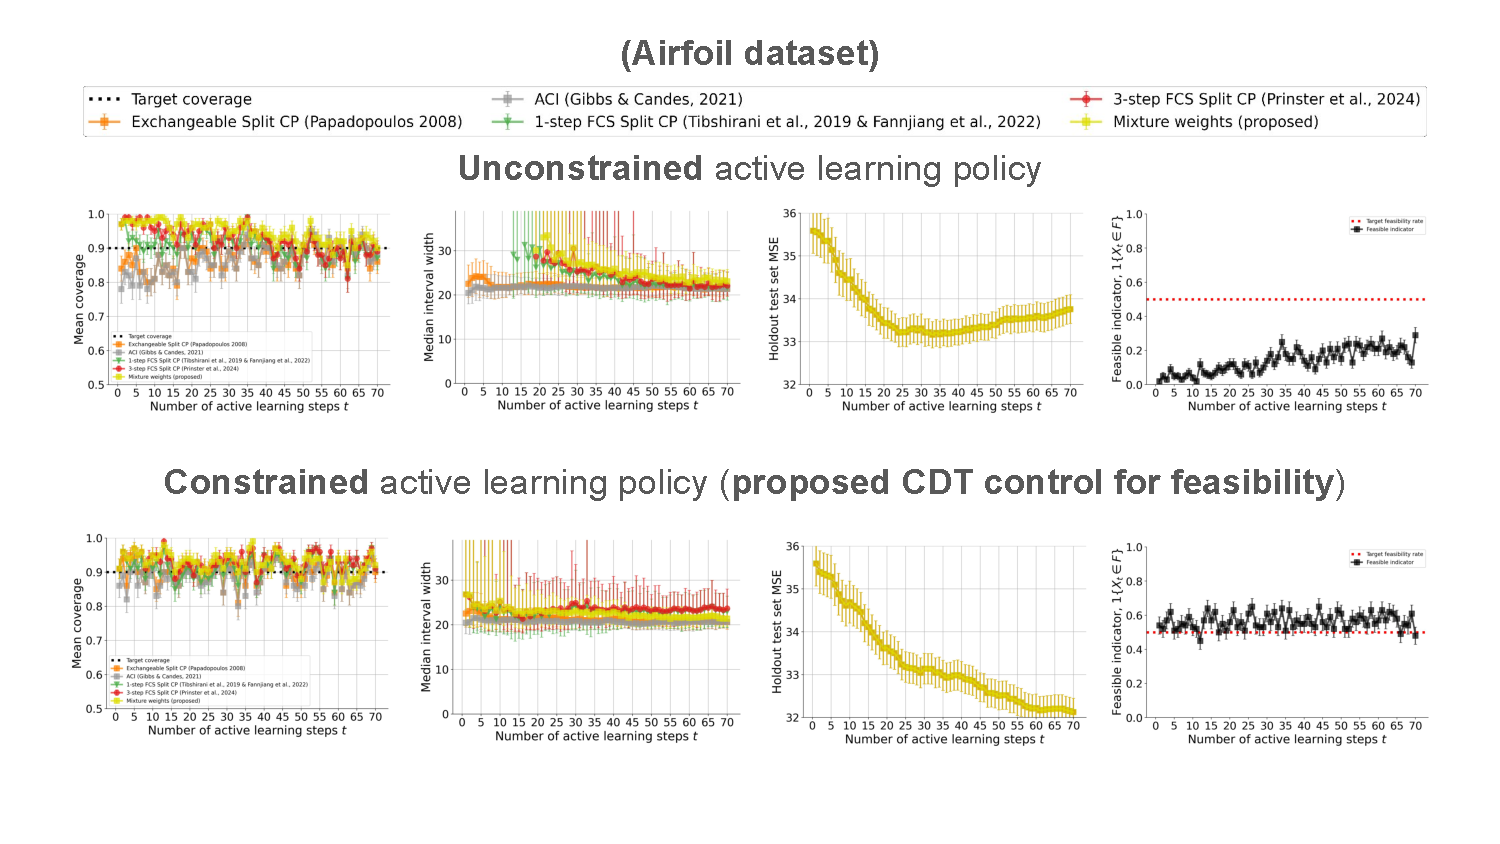
\includegraphics[width=0.85\textwidth]{figures/airfoil.pdf}
    \caption{Results for airfoil UCI dataset.}
\end{figure}







\section{Pseudocode}




\begin{algorithm}[htbp]
    \caption{Full algorithm.}
    \label{alg:full_algorithm}
    \begin{algorithmic}[1] % [1] enables line numbering
        \REQUIRE Initial safe policy and prompts, $\pi_{\theta_{0}}$ and $\mathbf{X}_{\text{prompt}}^{(0)}$; num. policy improvement steps, $T$. 
        % \Ensure Processed data $P$
        % \STATE accepted $\gets [\ ]$
        \STATE $\mathbf{X}_{\text{gen}}^{(0)} \sim \pi_{\theta_{0}}(\cdot\mid \mathbf{X}_{\text{prompt}}^{(0)})$ \COMMENT{Generate initial data input batch from safe policy.}
        \STATE $\mathbf{D}_{\text{gen}}^{(0)}\gets \{(\mathbf{x}, f(\mathbf{x})) : \mathbf{x}\in \mathbf{X}_{\text{gen}}^{(0)}\}$ \COMMENT{Label generated data batch.}
        \STATE $\mathbf{D}_{\text{cal}}^{(0)}\sim \mathbf{D}_{\text{gen}}^{(0)}$ \COMMENT{Sample initial cal. data (unif. w/o rep.) from generated.}
        \STATE $\mathbf{D}_{\text{train}}^{(0)}\gets \textsc{Select}(\mathbf{D}_{\text{gen}}^{(0)}\backslash\mathbf{D}_{\text{cal}}^{(0)})$ \COMMENT{Select initial training data from best non-cal data.}
        \STATE
        \STATE \# Initialize lists of policies, prompts, bounds, calibration data.
        \STATE $\pi^{(\text{all})}\gets [\pi_{\theta_0}]; \ \mathbf{X}_{\text{prompt}}^{(\text{all})}\gets [\mathbf{X}_{\text{prompt}}^{(0)} ];  \ \hat{\beta}^{(\text{all})}\gets [\infty]; \ \mathbf{D}_{\text{cal}}^{(\text{all})}\gets [\mathbf{D}_{\text{cal}}^{(0)}]$ 
        % \STATE $\mathbf{X}_{\text{prompt}}^{(\text{all})}\gets [\mathbf{X}_{\text{prompt}}^{(0)} ]$ \COMMENT{List of prompt sequences}
        % \STATE $\hat{\beta}^{(\text{all})}\gets [\infty]$ \COMMENT{List of all selected lik-ratio bounds}
        % \STATE $\mathcal{D}_{\text{safe}}^{(\text{all})} \gets [\ ]$ \COMMENT{List of safe policy proposal samples}
        % \STATE $\mathcal{D}_{\text{uncon}}^{(\text{all})} \gets [\ ]$ \COMMENT{List of unconstrained policy proposal samples}
        \STATE 
        \FOR{$t \in \{1, ..., T\}$}
            \STATE \# Learning: Prepare new ``unconstrained policy'' \& seeds
            \STATE $\theta_{t} \gets \textsc{Train}(\theta_{t-1}, \mathbf{D}_{\text{train}}^{(t-1)})$ \COMMENT{Learn new unconstrained policy.}
            \STATE $\mathbf{X}_{\text{prompt}}^{(t)} \gets \textsc{SelectX}(\mathbf{D}_{\text{train}}^{(t-1)})$ \COMMENT{Select seeds for unconstrained policy.}
            \STATE
            % \STATE \# Generate Proposals: Generate safe \& unconstrained proposals for policy control.
            % \STATE $\mathbf{X}_{\text{safe}}^{(t)} \sim \pi_{\theta_{t-1}}^{(\hat{\beta}_{t-1})}(\cdot\mid \mathbf{X}_{\text{prompt}}^{(t-1)})$ \COMMENT{Generate proposals from last safe policy (use AR for $t>1$).}
            % \STATE $\mathbf{X}_{\text{uncon}}^{(t)} \sim \pi_{\theta_{t}}(\cdot\mid \mathbf{X}_{\text{prompt}}^{(t)})$ \COMMENT{Generate proposals from current unconstrained policy.}
            % \STATE
            \STATE \# Policy Control
            \STATE $\pi_{\theta_{t}}^{(\hat{\beta}_t)},\ \hat{\beta}_t, \hat{\psi}_t \gets \textsc{ConformalPolicyControl}\big(\pi^{(\text{all})}, \mathbf{X}_{\text{prompt}}^{(\text{all})}, \hat{\beta}^{(\text{all})}, \mathbf{D}_{\text{cal}}^{(\text{all})}\big)$
            % \STATE $\pi_{\theta_{t}}^{(\hat{\beta}_t)} \gets \textsc{PolicyControl}\big(\pi_{\theta_{t-1}}^{(\hat{\beta}_{t-1})}(\cdot\mid \mathbf{X}_{\text{prompt}}^{(t-1)}), \mathbf{X}_{\text{safe}}^{(t)}, \pi_{\theta_{t}}(\cdot\mid \mathbf{X}_{\text{prompt}}^{(t)}), \mathbf{X}_{\text{uncon}}^{(t)}\big)$
            % \STATE $\pi_{\theta_{t}}^{(\hat{\beta}_t)}(\cdot\mid \mathbf{X}_{\text{prompt}}^{(t)}) \gets \textsc{MakeAcceptRejectAlgo}()$ 
            \STATE
            \STATE \# Generation \& Labeling
            \STATE $\mathbf{X}_{\text{gen}}^{(t)} \sim \pi_{\theta_{t}}^{(\hat{\beta}_t)}(\cdot \mid \mathbf{X}_{\text{prompt}}^{(t)})$
            \STATE $\mathbf{D}_{\text{gen}}^{(t)}\gets \{(\mathbf{x}, f(\mathbf{x})) : \mathbf{x}\in \mathbf{X}_{\text{gen}}^{(t)}\}$ \COMMENT{Label generated data batch.}
            \STATE
            \STATE \# Prepare calibration \& training data for next round.
            \STATE $\mathbf{D}_{\text{cal}}^{(t)}\sim \mathbf{D}_{\text{gen}}^{(t)}$ \COMMENT{Sample cal. data (unif. w/o rep.) from generated.}
            \STATE $\mathbf{D}_{\text{train}}^{(t)}\gets \textsc{Select}(\mathbf{D}_{\text{gen}}^{(t)}\backslash\mathbf{D}_{\text{cal}}^{(t)})$ \COMMENT{Select training data from best non-cal data.}
        \ENDFOR
        \STATE  accepted
    \end{algorithmic}
\end{algorithm}


\begin{algorithm}[htbp]
    \caption{\textsc{ConformalPolicyControl}$(\pi_{\theta_{0:t}}, \mathbf{X}_{\text{prompt}}^{(0:t)}, \hat{\beta}^{(0:t-1)}, \hat{\psi}^{(0:t-1)}, \mathbf{D}_{\text{cal}}^{(0:t-1)}, \textit{Liks}_{\text{cal}}^{(\hat{\beta}_{0:(t-1)})})$}
    \label{alg:conformal_policy_control}
    \begin{algorithmic}[1] % [1] enables line numbering
        \REQUIRE Policies list, $\pi^{(\text{all})}$; prompt batches list, $\mathbf{X}_{\text{prompt}}^{(\text{all})}$; lik-ratio bounds list, $\hat{\beta}^{(\text{all})}$; cal data list, $\mathbf{D}_{\text{cal}}^{(\text{all})}$.
        % \STATE \# Generate Proposals: Generate safe \& unconstrained proposals for policy control.
        \STATE $\textbf{X}^{(t)}_{\text{prop\_all}}\gets [\ ]$ \COMMENT{List to store proposals}
        \STATE 
        \STATE \# Outer for loop: First try using unconstrained policy as proposal before going to safe policy
        \FOR {$i, \pi(\cdot \mid \mathbf{X}) \in \textsc{enumerate}\big(\big[\pi_{\theta_{t}}(\cdot\mid \mathbf{X}_{\text{prompt}}^{(t)}), \pi_{\theta_{t-1}}^{(\hat{\beta}_{t-1})}(\mathbf{x}\mid \mathbf{X}_{\text{prompt}}^{(t-1)})\big]\big)$}
            \STATE $\textit{proposal}\gets [\textit{`unconstrained'} \ \textbf{if} \ i == 0 \ \textbf{else} \ \textit{`safe'}]$ \COMMENT{Which policy using as proposal}
            \STATE
            \STATE \# Compute unconstrained-over-safe lik-ratios and grid to search over
            % \STATE \# Construct grid of lik-ratio bounds to search over, using safe \& unconstrained proposal samples
            % \STATE $\mathbf{X}_{\text{safe}}^{(t)} \sim \pi_{\theta_{t-1}}^{(\hat{\beta}_{t-1})}(\cdot\mid \mathbf{X}_{\text{prompt}}^{(t-1)})$ \COMMENT{Generate proposals from last safe policy.}
            % \STATE $\mathbf{X}_{\text{prop}}^{(t)} \sim \pi(\cdot\mid \mathbf{X})$; \quad $\textbf{X}^{(t)}_{\text{prop\_all}}.\textsc{append}(\textbf{X}^{(t)}_{\text{prop}})$ \COMMENT{Generate and store proposals.}
            % \STATE $\textit{Liks}_{\text{prop}}^{(0:t)}\gets \textsc{ComputeUnconstrainedLiksAllModels}\big(\mathbf{X}_{\text{prop}}^{(t)}, \pi^{(\text{all})}, \mathbf{X}_{\text{prompt}}^{(\text{all})}\big)$
            % \STATE $\textit{Liks}_{\text{prop}}^{(\hat{\beta}_{0:t-1})}\gets \textsc{ConstrainLiks}\big(\textit{Liks}_{\text{prop}}^{(0:(t-1))}, \hat\beta_{0:(t-1)}, \hat\psi_{0:(t-1)}\big)$
            \IF {$\textit{proposal} == \textit{`unconstrained'}$}
                \STATE $(\hat{\beta}_{t}, \hat\psi_{t}) \gets (\infty, 1)$
                % \STATE $\mathbf{X}_{\text{prop}}^{(t)}, \textit{Liks}_{\text{prop}}^{(0:t)}, \textit{Liks}_{\text{prop}}^{(\hat{\beta}_{0:t-1})}\gets \textsc{ARSampleAndGetLiks}\big(\pi_{\theta_{0:t}},  \mathbf{X}_{\text{prompt}}^{(0:t)}, \hat{\beta}_{0:t}, \hat\psi_{0:t}, n_t\big)$
            \ELSE
                \STATE $(\hat{\beta}_{t}, \hat\psi_{t}) \gets (\textit{sys.float\_info.min}, \textit{sys.float\_info.min})$
            \ENDIF
            \STATE $\mathbf{X}_{\text{prop}}^{(t)}, \textit{Liks}_{\text{prop}}^{(0:t)}, \textit{Liks}_{\text{prop}}^{(\hat{\beta}_{0:t})}\gets \textsc{ARSampleAndGetLiks}\big(\pi_{\theta_{0:t}},  \mathbf{X}_{\text{prompt}}^{(0:t)}, \hat{\beta}_{0:t}, \hat\psi_{0:t}, n_t\big)$
            % \STATE $\mathbf{X}_{\text{prop}}^{(t)}, \textit{Liks}_{\text{prop}}^{(0:t)}, \textit{Liks}_{\text{prop}}^{(\hat{\beta}_{0:t-1})}\gets \textsc{ARSampleAndGetLiks}\big(\pi_{\theta_{0:t}},  \mathbf{X}_{\text{prompt}}^{(0:t)}, \hat{\beta}_{0:t-1}, \hat\psi_{0:t-1}, n_t\big)$
            % \STATE $\textbf{X}^{(t)}_{\text{prop\_all}}.\textsc{append}(\textbf{X}^{(t)}_{\text{prop}})$
            % \STATE $V_{\text{prop}}^{(t)} \gets \big\{\pi_{\theta_{t}}(\mathbf{x}\mid \mathbf{X}_{\text{prompt}}^{(t)})/\pi_{\theta_{t-1}}^{(\hat{\beta}_{t-1})}(\mathbf{x}\mid \mathbf{X}_{\text{prompt}}^{(t-1)}) : \mathbf{x} \in \mathbf{X}_{\text{prop}}^{(t)}\big\}$ \COMMENT{Get set of lik-ratio values}
            \STATE $V_{\text{prop}}^{(t)} \gets \textit{Liks}_{\text{prop}}^{(t)}/\textit{Liks}_{\text{prop}}^{(\hat{\beta}_{t-1})}$ \COMMENT{Get set of lik-ratio values}
            \STATE $G \gets \textsc{PrepareGrid}(V_{\text{prop}}^{(t)}, \textit{n\_grid}=\textit{n\_grid}, \textit{proposal}=\textit{proposal})$ 
            \STATE
            \STATE \# Compute mixture likelihoods for all cal and prop data
            \STATE $\textit{MixProps} \gets \textsc{GetMixProportions}(\mathbf{D}_{\text{cal}}^{(0:t-1)})$
            \STATE $\textit{MixLiks}_{\text{cal}}^{(\hat{\beta}_{0:(t-1)})} \gets \textsc{ComputeMixLiks}(\textit{MixLiks}_{\text{cal}}^{(\hat{\beta}_{0:(t-1)})}, \textit{MixProps})$
            \STATE $\textit{MixLiks}_{\text{prop}}^{(\hat{\beta}_{0:(t-1)})} \gets \textsc{ComputeMixLiks}(\textit{MixLiks}_{\text{prop}}^{(\hat{\beta}_{0:(t-1)})}, \textit{MixProps})$
            \STATE
            \STATE \# Search for largest bound in grid that satisfies conformal constraint
            \FOR{$\beta_t \in G$}
                \STATE
                \STATE \# Estimate normalizing constant via IWMCI
                % \STATE $\textit{LRs}_{\text{prop}}^{(t)} \gets $
                \STATE $\hat{\psi}_t \gets \textsc{IWMCI}(V_{\text{prop}}^{(t)}, \beta_t)$
                \STATE
                \STATE \# Compute constrained likelihoods for cal \& prop data on current candidate $\beta_t$ 
                \STATE $\textit{Liks}_{\text{cal}}^{(\beta_t)}\gets \textsc{ConstrainLiks}\big(\textit{Liks}_{\text{cal}}^{((t-1):t)}, \hat\beta_{(t-1):t}, \hat\psi_{(t-1):t}\big)$
                \STATE $\textit{Liks}_{\text{prop}}^{(\beta_t)}\gets \textsc{ConstrainLiks}\big(\textit{Liks}_{\text{prop}}^{((t-1):t)}, \hat\beta_{(t-1):t}, \hat\psi_{(t-1):t}\big)$
                \STATE
                \STATE \# Compute CP (mixture) weights for $\beta_t$
                \STATE $w_{\text{cal}} \gets \textit{Liks}_{\text{cal}}^{(\beta_t)} / \textit{MixLiks}_{\text{cal}}^{(\hat{\beta}_{0:(t-1)})}$
                % \FOR{$\mathbf{x_i} \in \mathbf{D_{\text{cal}}^{(\text{all})}}$}
                %     \STATE $w.\textsc{append}\big((\pi_{\theta_{t}}^{(\beta_t)}(\mathbf{x_i}\mid \mathbf{X}_{\text{prompt}}^{(t)})/\hat{\psi}_t)/\pi_{\theta_{1:t-1}}^{\text{mix}}(\mathbf{x_i})\big)$ \COMMENT{Norm const est. via IWMCI}
                % \ENDFOR
                \STATE 
                \STATE \# Compute test point weight
                \STATE
                $w_{\text{test}} \gets \sum\Big((\textit{Liks}_{\text{prop}}^{(\beta_t)})^2 / \textit{MixLiks}_{\text{prop}}^{(\hat{\beta}_{0:(t-1)})}\Big)$
                % $w_{\text{test}} \gets \sum\Big(\big\{(\pi_{(\theta_{t}}^{(\beta_t)}(\mathbf{x}\mid \mathbf{X}_{\text{prompt}}^{(t)})/\hat{\psi}_t)^2/\pi_{\theta_{1:t-1}}^{\text{mix}}(\mathbf{x}) : \mathbf{x} \in \mathbf{X}_{\text{safe}}^{(t)}\cup\mathbf{X}_{\text{uncon}}^{(t)}\big\}\Big)$
                \STATE
                \STATE \# Concatenate and normalize
                \STATE $\tilde{w} \gets (w_{\text{cal}}, w_{\text{test}}) / (\sum_{w_i\in w_{\text{cal}}}(w_i)+w_{\text{test}})$ \COMMENT{Normalize}
                \STATE
                \STATE \# Check if constraint is satisfied
                \IF {$\sum_{i\in\mathcal{D}_{\text{cal}}}\tilde{w}_i\cdot\mathbbm{1}\{x'_{i}\not\in\mathcal{F}\}+2\tilde{w}_{\text{test}} \leq \alpha$}
                    \STATE $\hat{\beta}_t \gets \beta_t$
                    \STATE $\pi_{\theta_{t}}^{(\hat{\beta}_t)}(\cdot\mid \mathbf{X}_{\text{prompt}}^{(t)}).\textsc{ConstrainLiks} \gets \textsc{ConstrainLiks}(\cdot \ ; \pi^{\text{(all)}}, \mathbf{X}_{\text{prompt}}^{(\text{all})}, \hat{\beta}^{(\text{all})}, \psi^{(\text{all})}, t)$
                    \STATE $\pi_{\theta_{t}}^{(\hat{\beta}_t)}(\cdot\mid \mathbf{X}_{\text{prompt}}^{(t)}).\textsc{Generator} \gets \textsc{Generator}(\cdot \ ; \pi_{\theta_{t-1}}^{(\hat{\beta}_{t-1})},  \mathbf{X}_{\text{prompt}}^{(t-1)}, \pi_{\theta_{t}}, \mathbf{X}_{\text{prompt}}^{(t)}, \hat{\beta}_t)$
                    \STATE  $\beta_t$
                \ENDIF
            \ENDFOR
            % \STATE
            % \STATE \# Construct grid of lik-ratio bounds to search over, using safe \& unconstrained proposal samples
            % \STATE $\mathbf{X}_{\text{safe}}^{(t)} \sim \pi_{\theta_{t-1}}^{(\hat{\beta}_{t-1})}(\cdot\mid \mathbf{X}_{\text{prompt}}^{(t-1)})$ \COMMENT{Generate proposals from last safe policy.}
        \ENDFOR
    \end{algorithmic}
\end{algorithm}




% \begin{algorithm}[htbp]
%     \caption{\textsc{ConformalPolicyControl}($\pi^{(\text{all})}, \mathbf{X}_{\text{prompt}}^{(\text{all})}, \hat{\beta}^{(\text{all})}, \mathbf{D}_{\text{cal}}^{(\text{all})}$)}
%     \label{alg:conformal_policy_control}
%     \begin{algorithmic}[1] % [1] enables line numbering
%         \REQUIRE Policies list, $\pi^{(\text{all})}$; prompt batches list, $\mathbf{X}_{\text{prompt}}^{(\text{all})}$; lik-ratio bounds list, $\hat{\beta}^{(\text{all})}$; cal data list, $\mathbf{D}_{\text{cal}}^{(\text{all})}$.
%         % \STATE \# Generate Proposals: Generate safe \& unconstrained proposals for policy control.
%         \STATE $\textbf{X}^{(t)}_{\text{prop\_all}}\gets [\ ]$ \COMMENT{List to store proposals}
%         \STATE 
%         \STATE \# Outer for loop: First try using unconstrained policy as proposal before going to safe policy
%         \FOR {$i, \pi(\cdot \mid \mathbf{X}) \in \textsc{enumerate}\big(\big[\pi_{\theta_{t}}(\cdot\mid \mathbf{X}_{\text{prompt}}^{(t)}), \pi_{\theta_{t-1}}^{(\hat{\beta}_{t-1})}(\mathbf{x}\mid \mathbf{X}_{\text{prompt}}^{(t-1)})\big]\big)$}
%             \STATE $\textit{proposal}\gets [\textit{`unconstrained'} \ \textbf{if} \ i == 0 \ \textbf{else} \ \textit{`safe'}]$ \COMMENT{Which policy using as proposal}
%             \STATE
%             \STATE \# Compute unconstrained-over-safe lik-ratios and grid to search over
%             % \STATE \# Construct grid of lik-ratio bounds to search over, using safe \& unconstrained proposal samples
%             % \STATE $\mathbf{X}_{\text{safe}}^{(t)} \sim \pi_{\theta_{t-1}}^{(\hat{\beta}_{t-1})}(\cdot\mid \mathbf{X}_{\text{prompt}}^{(t-1)})$ \COMMENT{Generate proposals from last safe policy.}
%             \STATE $\mathbf{X}_{\text{prop}}^{(t)} \sim \pi(\cdot\mid \mathbf{X})$; \quad $\textbf{X}^{(t)}_{\text{prop\_all}}.\textsc{append}(\textbf{X}^{(t)}_{\text{prop}})$ \COMMENT{Generate and store proposals.}
%             \STATE $\textit{Liks}_{\text{prop}}^{(0:t)}\gets \textsc{ComputeUnconstrainedLiksAllModels}\big(\mathbf{X}_{\text{prop}}^{(t)}, \pi^{(\text{all})}, \mathbf{X}_{\text{prompt}}^{(\text{all})}\big)$
%             \STATE $\textit{Liks}_{\text{prop}}^{(\hat{\beta}_{t-1})}\gets \textsc{ConstrainLiks}\big(\textit{Liks}_{\text{prop}}^{(0:t)}[0:(t-1)], \hat\beta_{0:t}[0:(t-1)], \hat\psi_{0:t}[0:(t-1)]\big)$
%             % \STATE $\textbf{X}^{(t)}_{\text{prop\_all}}.\textsc{append}(\textbf{X}^{(t)}_{\text{prop}})$
%             % \STATE $V_{\text{prop}}^{(t)} \gets \big\{\pi_{\theta_{t}}(\mathbf{x}\mid \mathbf{X}_{\text{prompt}}^{(t)})/\pi_{\theta_{t-1}}^{(\hat{\beta}_{t-1})}(\mathbf{x}\mid \mathbf{X}_{\text{prompt}}^{(t-1)}) : \mathbf{x} \in \mathbf{X}_{\text{prop}}^{(t)}\big\}$ \COMMENT{Get set of lik-ratio values}
%             \STATE $V_{\text{prop}}^{(t)} \gets \textit{Liks}_{\text{prop}}^{(0:t)}[t,:]/\textit{Liks}_{\text{prop}}^{(\hat{\beta}_{t-1})}$ \COMMENT{Get set of lik-ratio values}
%             \STATE $G \gets \textsc{PrepareGrid}(V_{\text{prop}}^{(t)}, \textit{n\_grid}=\textit{n\_grid}, \textit{proposal}=\textit{proposal})$ 
%             \STATE
%             \STATE \# Search for largest bound in grid that satisfies conformal constraint
%             \FOR{$\beta_t \in G$}
%                 \STATE
%                 \STATE \# Estimate normalizing constant via IWMCI
%                 % \STATE $\textit{LRs}_{\text{prop}}^{(t)} \gets $
%                 \STATE $\hat{\psi}_t \gets \textsc{IWMCI}(V_{\text{prop}}^{(t)}, \beta_t)$
%                 \STATE
%                 \STATE \# Compute CP (mixture) weights for $\beta_t$
%                 \STATE $w \gets [\ ]$
%                 \FOR{$\mathbf{x_i} \in \mathbf{D_{\text{cal}}^{(\text{all})}}$}
%                     \STATE $w.\textsc{append}\big((\pi_{\theta_{t}}^{(\beta_t)}(\mathbf{x_i}\mid \mathbf{X}_{\text{prompt}}^{(t)})/\hat{\psi}_t)/\pi_{\theta_{1:t-1}}^{\text{mix}}(\mathbf{x_i})\big)$ \COMMENT{Norm const est. via IWMCI}
%                 \ENDFOR
%                 \STATE 
%                 \STATE \# Compute test point weight
%                 \STATE
%                 $w_{\text{test}} \gets \textsc{sum}\Big(\big\{(\pi_{(\theta_{t}}^{(\beta_t)}(\mathbf{x}\mid \mathbf{X}_{\text{prompt}}^{(t)})/\hat{\psi}_t)^2/\pi_{\theta_{1:t-1}}^{\text{mix}}(\mathbf{x}) : \mathbf{x} \in \mathbf{X}_{\text{safe}}^{(t)}\cup\mathbf{X}_{\text{uncon}}^{(t)}\big\}\Big)$
%                 \STATE $\tilde{w} \gets w / (\sum_{w_i\in w}(w_i)+w_{\text{test}})$ \COMMENT{Normalize}
%                 \STATE
%                 \STATE \# Check if constraint is satisfied
%                 \IF {$\sum_{i\in\mathcal{D}_{\text{cal}}}\tilde{w}_i\cdot\mathbbm{1}\{x'_{i}\not\in\mathcal{F}\}+2\tilde{w}_{\text{test}} \leq \alpha$}
%                     \STATE $\hat{\beta}_t \gets \beta_t$
%                     \STATE $\pi_{\theta_{t}}^{(\hat{\beta}_t)}(\cdot\mid \mathbf{X}_{\text{prompt}}^{(t)}).\textsc{ConstrainLiks} \gets \textsc{ConstrainLiks}(\cdot \ ; \pi^{\text{(all)}}, \mathbf{X}_{\text{prompt}}^{(\text{all})}, \hat{\beta}^{(\text{all})}, \psi^{(\text{all})}, t)$
%                     \STATE $\pi_{\theta_{t}}^{(\hat{\beta}_t)}(\cdot\mid \mathbf{X}_{\text{prompt}}^{(t)}).\textsc{Generator} \gets \textsc{Generator}(\cdot \ ; \pi_{\theta_{t-1}}^{(\hat{\beta}_{t-1})},  \mathbf{X}_{\text{prompt}}^{(t-1)}, \pi_{\theta_{t}}, \mathbf{X}_{\text{prompt}}^{(t)}, \hat{\beta}_t)$
%                     \STATE \RETURN $\beta_t$
%                 \ENDIF
%             \ENDFOR
%             % \STATE
%             % \STATE \# Construct grid of lik-ratio bounds to search over, using safe \& unconstrained proposal samples
%             % \STATE $\mathbf{X}_{\text{safe}}^{(t)} \sim \pi_{\theta_{t-1}}^{(\hat{\beta}_{t-1})}(\cdot\mid \mathbf{X}_{\text{prompt}}^{(t-1)})$ \COMMENT{Generate proposals from last safe policy.}
%         \ENDFOR
%     \end{algorithmic}
% \end{algorithm}





\begin{algorithm}[htbp]
    \caption{\textsc{PrepareGrid}($V, \textit{n\_grid}, \textit{proposal}$) $\rightarrow G$ \\ Prepare grid of descending values with desired coarseness.}
    \label{alg:conformal_policy_control}
    \begin{algorithmic}[1] % [1] enables line numbering
        \REQUIRE Input values, $V$; approximate desired number of values in grid, $\textit{n\_grid}$; variable indicating which policy is used as the proposal, $\textit{proposal}\in [\textit{`unconstrained'}, \textit{`safe'}]$.
            \STATE
            \STATE \# Construct grid of lik-ratio bounds to search over
            % \STATE $\mathbf{X}_{\text{uncon}}^{(t)} \sim \pi_{\theta_{t}}(\cdot\mid \mathbf{X}_{\text{prompt}}^{(t)})$ \COMMENT{Generate proposals from current unconstrained policy.}
            \STATE $G \gets \textsc{SortDescending}\big(V\big)$
            \IF{$\textit{proposal}==\textit{`unconstrained'}$} 
                \STATE \# Construct grid for proposals from unconstrained policy
                \STATE $G \gets G[G > 1]$
                \STATE $G \gets \textsc{GetEveryKthElement}(G, k=\text{len}(G)/\text{n\_grid})$ \COMMENT{Coarsen grid for efficiency}
                \STATE $G\gets \textsc{Concatenate}((\infty, G, 1))$ \COMMENT{Append $\infty$ \& 1}
            \ELSE
                \STATE \# Construct grid for proposals from safe policy
                \STATE $G \gets G[G< 1]$
                \STATE $G \gets \textsc{GetEveryKthElement}(G, k=\text{len}(G)/\text{n\_grid})$ \COMMENT{Coarsen grid for efficiency}
                \STATE $G\gets \textsc{Concatenate}((G, \textsc{sys.float\_info.min}))$ \COMMENT{Append smallest positive float value}
            \ENDIF
            \STATE  $G$
            % \STATE $G \gets [G_{i*\text{len}(G')} \quad \textbf{for} \quad i \in \{0, 1, ..., k\}]$ \COMMENT{}
        \STATE
    \end{algorithmic}
\end{algorithm}

% \begin{algorithm}[htbp]
%     \caption{\textsc{GetAcceptRejectSampler}\big($\pi_{\theta_{t-1}}^{(\hat{\beta}_{t-1})},  \mathbf{X}_{\text{prompt}}^{(t-1)}, \pi_{\theta_{t}}, \mathbf{X}_{\text{prompt}}^{(t)}, \hat{\beta}_t$\big) \\ Sample from constrained policy, $\pi_{\theta_t}^{(\hat{\beta}_t)}(\cdot\mid\mathbf{X}_{\text{prompt}}^{(t)})$.}
%     \label{alg:rej_sampling_constrained_policy}
%     \begin{algorithmic}[1] % [1] enables line numbering
%         \REQUIRE Safe policy $\pi_{\theta_{t-1}}^{(\hat{\beta}_{t-1})}(\cdot\mid \mathbf{X}_{\text{prompt}}^{(t-1)})$, unconstrained policy $\pi_{\theta_{t}}(\cdot\mid \mathbf{X}_{\text{prompt}}^{(t)})$, lik-ratio bound $\hat{\beta}_t$, num target $n_t$. 
%         % \Ensure Processed data $P$
%         \STATE \Function{AcceptRejectSampler}{$\cdot, n_t$ ; }
%         \STATE accepted $\gets [\ ]$
%         \IF {$\beta_t\leq 1$} \COMMENT{Use safe policy, $\pi_{\theta_{t-1}}^{(\hat{\beta}_{t-1})}(\cdot)$, as proposal}
%             \WHILE {len(accepted) $< n_t$}
%                 \STATE $x_t\sim \pi_{\theta_{t-1}}^{(\hat{\beta}_{t-1})}(\cdot)$  
%                 \STATE $u \sim \text{Unif}[0, 1]$
%                 \IF {$u < \pi_{\theta_t}(x_t) / (\beta_t \pi_{\theta_{t-1}}^{(\hat{\beta}_{t-1})}(x_t))$}
%                     \STATE accepted.append($x_t$)
%                 \ENDIF
%             \ENDWHILE
%         \ELSE \COMMENT{Use unconstrained policy, $\pi_{\theta_{t}}(\cdot)$, as proposal}
%             \WHILE {len(accepted) $< n_t$}
%                 \STATE $x_t\sim \pi_{\theta_{t}}(\cdot)$  
%                 \STATE $u \sim \text{Unif}[0, 1]$
%                 \IF {$u < \beta_t \pi_{\theta_{t-1}}^{(\hat{\beta}_{t-1})}(x_t)/ \pi_{\theta_t}(x_t)$}
%                     \STATE accepted.append($x_t$)
%                 \ENDIF
%             \ENDWHILE
%         \ENDIF
%         \STATE \RETURN accepted
%         \EndFunction
%         \STATE $\pi_{\theta_t}^{(\hat{\beta}_t)}(\cdot\mid\mathbf{X}_{\text{prompt}}^{(t)}) \gets \textsc{AcceptRejectSampler}$
%         \STATE \RETURN $\pi_{\theta_t}^{(\hat{\beta}_t)}(\cdot\mid\mathbf{X}_{\text{prompt}}^{(t)})$
%     \end{algorithmic}
% \end{algorithm}



\begin{algorithm}[htbp]
    \caption{\textsc{IWMCI}($\textit{LRs}, \beta_t$) \\
    Importance-Weighted Monte Carlo Integration estimation of $\int_{\Omega}\pi_{\theta_t}^{(\beta_t)}(x)\text{d}x$.}
    \label{alg:rej_sampling_constrained_policy}
    \begin{algorithmic}[1] % [1] enables line numbering
        \REQUIRE Lik-ratios (unconstrained over safe) of proposal samples, $V$; lik-ratio bound, $\beta_t$.
        % ; variable indicating which policy is used as the proposal, $\textit{proposal}\in [\textit{`unconstrained'}, \textit{`safe'}]$.
        \STATE $\textit{LRs}(\beta_t)\gets [\ ]$ \COMMENT{List to store LRs (constrained over proposal) of proposed samples}
        \IF {$\beta_t\geq 1$} %\COMMENT{Use safe policy to estimate}
            \STATE \# If $\beta_t\geq 1$, assumes proposal is unconstrained.
            \FOR {$V_i \in V$}
                % \STATE LRs.append\big($\min\big(\beta_t\pi_{\theta_{t-1}}^{(\hat{\beta}_{t-1})}(x_i)/\pi_{\theta_{t}}(x_i),\ 1\big)$\big)
                \STATE $\textit{LRs}{(\beta_t)}$.\textsc{append}\big($\min(\beta_t/V_i,\ 1)$\big)
            \ENDFOR
        \ELSE %\COMMENT{Use unconstrained policy to estimate}
            \STATE \# Else, $\beta_t< 1$, and assume proposal is safe.
            \FOR {$V_i \in V$}
                \STATE $\textit{LRs}{(\beta_t)}$.\textsc{append}\big($\min(V_i,\ \beta_t)$\big)
            \ENDFOR
        \ENDIF
        \STATE  \textsc{mean}(\textit{LRs}$(\beta_t)$)
    \end{algorithmic}
\end{algorithm}



\begin{algorithm}[htbp]
    \caption{\textsc{ARSampleAndGetLiks}\big($\pi_{\theta_{0:t}},  \mathbf{X}_{\text{prompt}}^{(0:t)}, \hat{\beta}_{0:t}, \hat{\psi}_{0:t}, n_t$\big) \\ Sample from constrained policy, $\pi_{\theta_t}^{(\hat{\beta}_t)}(\cdot\mid\mathbf{X}_{\text{prompt}}^{(t)})$.}
    \label{alg:rej_sampling_constrained_policy}
    \begin{algorithmic}[1] % [1] enables line numbering
        % \REQUIRE Safe policy $\pi_{\theta_{t-1}}^{(\hat{\beta}_{t-1})}(\cdot\mid \mathbf{X}_{\text{prompt}}^{(t-1)})$, unconstrained policy $\pi_{\theta_{t}}(\cdot\mid \mathbf{X}_{\text{prompt}}^{(t)})$, lik-ratio bound $\hat{\beta}_t$, num target $n_t$. 
        % \Ensure Processed data $P$
        % \STATE \Function{AcceptRejectSampler}{$\cdot, n_t$ ; }
        \STATE $\mathbf{X}_{\text{accept}}^{(t)}\gets [\ ]$ \COMMENT{List to store accepted samples}
        % \STATE $\textit{V}_{\text{accept}}^{(t)} \gets [\ ]$ \COMMENT{List to store LRs (unconstrained over safe) for accepted samples}
        
        \IF {$\beta_t\geq 1$} 
            \STATE \# Use unconstrained policy, $\pi_{\theta_{t}}(\cdot)$, as proposal
            \WHILE{$\text{len}(\mathbf{X}_{\text{accept}}^{(t)}) < n_t$}
                % \STATE \# Choosing num proposals to try to avoid multiple batch generations
                % \STATE $n_{\text{prop}} \gets \text{int}(1.1\cdot\max(\hat\beta_{t}, 1/\hat\beta_{t})\cdot n_t)$ 
                % \STATE 
                \STATE \# Sample using model, ie using \textsc{run\_iterative\_generation}
                \STATE $\mathbf{X}_{\text{prop}}^{(t)}\sim \pi_{\theta_{t}}(\cdot)$ \COMMENT{Sample $n_{\text{prop}}$ from unconstrained policy as proposals} %\textsc{ARSampler}\big(\pi_{\theta_{0:(t-1)}},  \mathbf{X}_{\text{prompt}}^{(0:(t-1))}, \hat{\beta}_{0:(t-1)}, n_{\text{prop}}\big)$
                \STATE $\textit{Liks}_{\text{prop}}^{(0:t)}\gets \textsc{ComputeUnconstrainedLiksAllModels}\big(\mathbf{X}_{\text{prop}}^{(t)}, \pi^{(\text{all})}, \mathbf{X}_{\text{prompt}}^{(\text{all})}\big)$
                \STATE $\textit{Liks}_{\text{prop}}^{(\hat{\beta}_{0:t})}\gets \textsc{ConstrainLiks}\big(\textit{Liks}_{\text{prop}}^{(0:t)}, \hat\beta_{0:t}, \hat\psi_{0:t}\big)$
                \STATE $V_{\text{prop}}^{(t)} \gets \textit{Liks}_{\text{prop}}^{(t)}/\textit{Liks}_{\text{prop}}^{(\hat{\beta}_{t-1})}$ \COMMENT{Get set of lik-ratio values}
                % \STATE
                % \STATE $x_t\sim \pi_{\theta_{t}}(\cdot)$  
                % \STATE $u \sim \text{Unif}[0, 1]$
                % \IF {$u < \beta_t \pi_{\theta_{t-1}}^{(\hat{\beta}_{t-1})}(x_t)/ \pi_{\theta_t}(x_t)$}
                %     \STATE $\mathbf{X}_{\text{accept}}^{(t)}.\textsc{append}(x_t)$
                % \ENDIF
                \STATE
                \STATE \# Accept or reject each proposal
                \FOR{$i, \mathbf{x_i}\in \textsc{enumerate}(\mathbf{X}_{\text{prop}}^{(t)})$}
                    \STATE $u \sim \text{Unif}[0, 1]$
                    % \IF {$u < \pi_{\theta_t}(x_t) / (\beta_t \pi_{\theta_{t-1}}^{(\hat{\beta}_{t-1})}(x_t))$}
                    \IF {$u < \beta_t/V_{\text{prop}}^{(t)}[i]$}
                    \STATE $\mathbf{X}_{\text{accept}}^{(t)}.\textsc{append}(\mathbf{x_i})$
                    \STATE $V_{\text{accept}}^{(t)}.\textsc{append}(V_{\text{prop}}^{(t)}[i])$
                        \IF{$\text{len}(\mathbf{X}_{\text{accept}}^{(t)})\geq n_t$}
                            \STATE \textbf{break}
                        \ENDIF
                    \ENDIF
                \ENDFOR
            \ENDWHILE
        \ELSE 
        \STATE \COMMENT{Use safe policy, $\pi_{\theta_{t-1}}^{(\hat{\beta}_{t-1})}(\cdot)$, as proposal}
            \WHILE {$\text{len}(\mathbf{X}_{\text{accept}}^{(t)}) < n_t$}
                % \STATE \# Choosing num proposals to try to avoid multiple batch generations
                % \STATE $n_{\text{prop}} \gets \text{int}(1.1\cdot\max(\hat\beta_{t-1}, 1/\hat\beta_{t-1})\cdot n_t)$ 
                % \STATE
                \STATE \# Recusively sample from previous constrained policy
                % \STATE $\mathbf{X}_{\text{prop}}^{(t)}\sim \textsc{ARSampler}\big(\pi_{\theta_{0:(t-1)}},  \mathbf{X}_{\text{prompt}}^{(0:(t-1))}, \hat{\beta}_{0:(t-1)}, n_{\text{prop}}\big)$
                % \STATE $\textit{Liks}_{\text{prop}}^{(0:t)}\gets \textsc{ComputeUnconstrainedLiksAllModels}\big(\mathbf{X}_{\text{prop}}^{(t)}, \pi^{(\text{all})}, \mathbf{X}_{\text{prompt}}^{(\text{all})}\big)$
                % \STATE $\textit{Liks}_{\text{prop}}^{(\hat{\beta}_{0:t})}\gets \textsc{ConstrainLiks}\big(\textit{Liks}_{\text{prop}}^{(0:t)}, \hat\beta_{0:t}, \hat\psi_{0:t}\big)$
                \STATE $\mathbf{X}_{\text{prop}}^{(t)}, \textit{Liks}_{\text{prop}}^{(0:t-1)}, \textit{Liks}_{\text{prop}}^{(\hat{\beta}_{0:t-1})}\gets\textsc{ARSampleAndGetLiks}\big(\pi_{\theta_{0:t-1}},  \mathbf{X}_{\text{prompt}}^{(0:t-1)}, \hat{\beta}_{0:t-1}, \hat{\psi}_{0:t-1}, n_t$\big)
                \STATE $\textit{Liks}_{\text{prop}}^{(t)}\gets \textsc{ComputeUnconstrainedLiksAllModels}\big(\mathbf{X}_{\text{prop}}^{(t)}, [\pi_{\theta_t}], [\mathbf{X}_{\text{prompt}}^{(t)}]\big)$
                \STATE $\textit{Liks}_{\text{prop}}^{(\hat{\beta}_{t})}\gets \textsc{ConstrainLiks}\big(\textit{Liks}_{\text{prop}}^{(t)}, \hat\beta_{t}, \hat\psi_{t}\big)$
                \STATE $V_{\text{prop}}^{(t)} \gets \textit{Liks}_{\text{prop}}^{(t)}/\textit{Liks}_{\text{prop}}^{(\hat{\beta}_{t-1})}$ \COMMENT{Get set of lik-ratio values}
                \STATE
                \STATE \# Accept or reject each proposal
                \FOR{$i, \mathbf{x_i}\in \textsc{enumerate}(\mathbf{X}_{\text{prop}}^{(t)})$}
                    \STATE $u \sim \text{Unif}[0, 1]$
                    % \IF {$u < \pi_{\theta_t}(x_t) / (\beta_t \pi_{\theta_{t-1}}^{(\hat{\beta}_{t-1})}(x_t))$}
                    \IF {$u < V_{\text{prop}}^{(t)}[i] / \beta_t$}
                    \STATE $\mathbf{X}_{\text{accept}}^{(t)}.\textsc{append}(\mathbf{x_i})$
                    % \STATE $V_{\text{accept}}^{(t)}.\textsc{append}(V_{\text{prop}}^{(t)}[i])$
                        \IF{$\text{len}(\mathbf{X}_{\text{accept}}^{(t)})\geq n_t$}
                            \STATE \textbf{break}
                        \ENDIF
                    \ENDIF
                \ENDFOR
                % \STATE $x_t\sim \pi_{\theta_{t-1}}^{(\hat{\beta}_{t-1})}(\cdot)$  
                % \STATE $u \sim \text{Unif}[0, 1]$
            \ENDWHILE
        \ENDIF
        \COMMENT{Save accepted samples' unconstrained likelihoods}
        \STATE $\textit{Liks}_{\text{accept}}^{(0:t)} \gets \textit{Liks}_{\text{prop}}^{(0:t)}[\mathbf{X}_{\text{prop}}^{(t)}\in\mathbf{X}_{\text{accept}}^{(t)}]$ 
        \STATE $\textit{Liks}_{\text{accept}}^{(\hat{\beta}_{0:t})} \gets \textit{Liks}_{\text{prop}}^{(\hat{\beta}_{0:t})}[\mathbf{X}_{\text{prop}}^{(t)}\in\mathbf{X}_{\text{accept}}^{(t)}]$ \COMMENT{Save accepted samples prev constrained liks}
        \STATE $\mathbf{X}_{\text{accept}}^{(t)}, \ \textit{Liks}_{\text{accept}}^{(0:t)}, \ \textit{Liks}_{\text{accept}}^{(\hat{\beta}_{0:t})}$
        % \EndFunction
        % \STATE $\pi_{\theta_t}^{(\hat{\beta}_t)}(\cdot\mid\mathbf{X}_{\text{prompt}}^{(t)}) \gets \textsc{AcceptRejectSampler}$
        % \STATE \RETURN $\pi_{\theta_t}^{(\hat{\beta}_t)}(\cdot\mid\mathbf{X}_{\text{prompt}}^{(t)})$
    \end{algorithmic}
\end{algorithm}





\begin{algorithm}[htbp]
    % \caption{\textsc{ConstrainLiks}$(\mathbf{x}, \pi^{\text{(all)}}, \mathbf{X}_{\text{prompt}}^{(\text{all})}, \hat{\beta}^{(\text{all})}, \psi^{(\text{all})}, t)$
    \caption{\textsc{ConstrainLiks}$(\textit{Liks}_{\text{prop}}^{(:t)}, \hat{\beta}_{:t}, \hat{\psi}_{:t})$
    \\
    }
    \label{alg:compute_likelihoods}
    \begin{algorithmic}[1] % [1] enables line numbering
        % \REQUIRE $\mathbf{x}, \pi^{\text{(all)}}, \mathbf{X}_{\text{prompt}}^{(\text{all})}, \hat{\beta}^{(\text{all})}, \psi^{(\text{all})}, t$.
        \REQUIRE $\textit{Liks}_{\text{prop}}^{(:t)} \in \mathbb{R}^{(*,n_{\text{prop}})}$: Matrix where each column has unconstrained likelihoods for times $..., t$ for a given proposal sample. 0th row will have \textit{constrained} likelihoods, which for time 0 are same as unconstrained (starting from initial safe policy); $\hat{\beta}_{:t}\in(0, \infty)^{*}:$ Bounds for times $ ..., t$; $\psi_{:t} \in (0, \infty)^{*}$: Normalization constants for times $ ..., t$.
        \STATE
        \STATE \# Get number of total models from last safe model to current model (inclusively). Main cases:
        \STATE \# if $\text{len}(\hat{\beta}_{:t})==t+1$, then running computation from start; and if $\text{len}(\hat{\beta}_{:t})==2$, then running 
        \STATE \# computation from most recent step.
        \STATE $n_{\text{models}} \gets \text{len}(\hat{\beta}_{:t})$ 
        \STATE $\textit{Liks}_{\text{prop}}^{(\hat{\beta}_{:t})} \gets \text{Zeros}((n_{\text{models}}, n_{\text{prop}}))$ \COMMENT{Matrix to store constrained likelihoods for all timesteps}
        \STATE $\textit{Liks}_{\text{prop}}^{(\hat{\beta}_{:t})}[0,:] \gets \textit{Liks}_{\text{prop}}^{(:t)}[0,:]$ \COMMENT{Initialize with last computed safe/constrained likelihoods}
        % \STATE $\pi^{(\hat{\beta})}(\mathbf{x}) \gets \big[\textit{Liks}_{\text{prop}}^{(:t)}[0,:]\big]$ \COMMENT{Initialize list to contain constrained likelihood at each time.}
        \STATE
        \STATE \# Compute \textit{constrained} likelihoods for each subsequent policy
        \FOR{$t'\in\{1, ..., n_{\text{models}}-1\}$}
            \STATE $\textit{Liks}_{\text{prop}}^{(\hat{\beta}_{:t})}[t',:] \gets \textsc{np.where}(\textit{Liks}_{\text{prop}}^{(:t)}[t',:]/\textit{Liks}_{\text{prop}}^{(\hat{\beta}_{:t})}[t'-1,:]<\beta_t,$ \\ 
            \qquad \qquad \qquad \qquad \qquad \qquad \qquad $\textit{Liks}_{\text{prop}}^{(:t)}[t',:]/\hat{\psi}_t, \quad \beta_t\cdot \textit{Liks}_{\text{prop}}^{(\hat{\beta}_{:t})}[t'-1,:]/\hat{\psi}_t)$
            % \IF {$\pi_{\theta_{t'}}(\mathbf{x}\mid \mathbf{X}_{\text{prompt}}^{(t')})/(\pi_{\theta_{t'-1}}^{(\beta_{t'-1})}(\mathbf{x}\mid \mathbf{X}_{\text{prompt}}^{(t'-1)})/\hat{\psi}_{t'-1}) < \beta_{t'}$}
            %     \STATE $\pi^{(\hat{\beta})}(\mathbf{x}).\textsc{append}\big(\pi_{\theta_{t'}}(\mathbf{x}\mid \mathbf{X}_{\text{prompt}}^{(t')}) / \psi_{t'}\big)$
            % \ELSE
            %     \STATE $\pi^{(\hat{\beta})}(\mathbf{x}).\textsc{append}\big(\beta_{t'}\cdot\pi^{(\hat{\beta})}(\mathbf{x})[-1] / \psi_{t'}\big)$
            % \ENDIF
        \ENDFOR
        \STATE $\textit{Liks}_{\text{prop}}^{(:t)}$ \COMMENT{Return all computed constrained likelihoods (last row is current timestep)} %$\pi^{(\hat{\beta})}(\mathbf{x})[-1]$ \COMMENT{Return last computed constrained likelihood (current timestep)}
    \end{algorithmic}
\end{algorithm}



% \begin{algorithm}[htbp]
%     \caption{\textsc{ConstrainLiks}$(\mathbf{x}, \pi^{\text{(all)}}, \mathbf{X}_{\text{prompt}}^{(\text{all})}, \hat{\beta}^{(\text{all})}, \psi^{(\text{all})}, t)$
%     \\
%     }
%     \label{alg:compute_likelihoods}
%     \begin{algorithmic}[1] % [1] enables line numbering
%         \REQUIRE $\mathbf{x}, \pi^{\text{(all)}}, \mathbf{X}_{\text{prompt}}^{(\text{all})}, \hat{\beta}^{(\text{all})}, \psi^{(\text{all})}, t$.
%         \STATE $\pi^{(\hat{\beta})}(\mathbf{x}) \gets \big[\pi_{\theta_0}(\mathbf{x}\mid \mathbf{X}_{\text{prompt}}^{(0)})\big]$ \COMMENT{Initialize list to contain constrained likelihood at each time.}
%         \STATE
%         \STATE \# Compute constrained likelihoods for each constrained policy
%         \FOR{$t'\in\{1, ..., t\}$}
%             \IF {$\pi_{\theta_{t'}}(\mathbf{x}\mid \mathbf{X}_{\text{prompt}}^{(t')})/(\pi_{\theta_{t'-1}}^{(\beta_{t'-1})}(\mathbf{x}\mid \mathbf{X}_{\text{prompt}}^{(t'-1)})/\hat{\psi}_{t'-1}) < \beta_{t'}$}
%                 \STATE $\pi^{(\hat{\beta})}(\mathbf{x}).\textsc{append}\big(\pi_{\theta_{t'}}(\mathbf{x}\mid \mathbf{X}_{\text{prompt}}^{(t')}) / \psi_{t'}\big)$
%             \ELSE
%                 \STATE $\pi^{(\hat{\beta})}(\mathbf{x}).\textsc{append}\big(\beta_{t'}\cdot\pi^{(\hat{\beta})}(\mathbf{x})[-1] / \psi_{t'}\big)$
%             \ENDIF
%         \ENDFOR
%         \STATE \RETURN $\pi^{(\hat{\beta})}(\mathbf{x})[-1]$ \COMMENT{Return last computed constrained likelihood (current timestep)}
%     \end{algorithmic}
% \end{algorithm}

% We want $\pi_{\theta_t}(x'\mid x)$ to maximize the expected improvement, $\max(f(x'_t)-f(x_t))$, while enforcing the risk constraint: $\mathbb{E}_{x'_t\sim \pi_{\theta_t}}[\mathbbm{1}\{x'_t\not\in\mathcal{F}\}\mid L_{<t}]\leq \alpha$. 

% (Approach based on conformal prediction with score for binary classifier)

% Say we have a prefit probabilistic classifier $\hat{\sigma}:\mathcal{X}\rightarrow[0, 1]$ for estimating the probability that a given sequence is feasible or not, that is, for estimating the probability $\mathbb{P}(x_t'\in \mathcal{F}\mid X=x_t')$. The nonconformity scores $V_i := \hat{s}:\mathcal{X}\times \{0, 1\}\rightarrow [0, 1]$ are $\hat{s}(X_i, Y_i)= (1 - \hat{\sigma}(X_i)) \cdot \mathbbm{1}\{X_i \in \mathcal{F}\} + \hat{\sigma}(X_i) \cdot (1-\mathbbm{1}\{X_i \in \mathcal{F}\})$, which are low (close to 0) when the correct class is predicted and high (close to 1) when the incorrect class is predicted. We can also separately 


% \begin{align}
%     \hat{s}(X_i, Y_i) := 
%     \begin{cases}
%         1 - \hat{\sigma}(X_i) \
%     \end{cases}
% \end{align}

% WTS:
% \begin{align}
%     \mathbb{P}(X_t \in \mathcal{F}) \geq 1-\alpha
% \end{align}


% LHS:
% \begin{align}
%     \mathbb{P}(X_t \in \mathcal{F}) := & \mathbb{P}(X_t \in \mathcal{F}\mid \hat{\sigma}(X_i)\geq \tau)\cdot \mathbb{P}(\hat{\sigma}(X_i)\geq \tau) \nonumber \\
%     & + \mathbb{P}(X_t \in \mathcal{F}\mid \hat{\sigma}(X_i) < \tau)\cdot \mathbb{P}(\hat{\sigma}(X_i) < \tau)
% \end{align}





% Let's say that the level $1-\alpha$ empirical quantile of the scores $V_{1:t}$ is $q_{1-\alpha}=\widehat{Q}_{1-\alpha}\{V_{1:t}\}$; then, we can say that a new test designed sequence $x_t'$ is feasible with confidence at least $1-\alpha$ if 
% \begin{align*}
%      q_{1-\alpha}
% \end{align*}

\newpage

\section{Theory}






\subsection{Conformal Policy Control for Batch Setting}
% \newtheorem{theorem}{Theorem}

\begin{theorem}
    
    \textit{(Conformal policy control guarantee for batch setting.)} The conformal policy control procedure satisfies
    \begin{align*}
        \mathbb{E}_{\hat{a}\sim p_t^{(\beta_t)}}\Big[L\big(Y_t, \hat{a}(X_t)\big)\Big] \leq \alpha.
    \end{align*}
    %Let $p_0$ denote a known ``safe'' policy, and let $p_t$ denote the learned policy at time $t$. Then, with $\beta_t\in [0, 1]$ denoting a mixture parameter such that $p_t^{(\beta_t)}:=\beta_tp_0 + (1-\beta_t)p_t$
    
\end{theorem}

Proof sketch: 
\begin{enumerate}
    \item Prove an oracle version of the CDT guarantee, assuming that the test point loss is known.
    \item Prove that a conservative adjustment is more conservative than the oracle version.
\end{enumerate}

\begin{proof}
    The following proof has some rough notation, but contains key steps. 
    Let $E_z^{(t)}$ denote the event of observing the multiset of data, that is denoting the event $\{Z_1, ..., Z_t\}=\{z_1, ..., z_t\}$; similarly let $E_l^{(t)}$ denote the event of observing the corresponding multiset of loss values, that is denoting the event $\{L_1, ..., L_t\}=\{l_1, ..., l_t\}$. Drawing from \citet{tibshirani2019conformal} and \citet{prinster2024conformal}, the probability that $L_t$ takes on the value $l_i$, conditional on $E_z^{(t)}$ (or, equivalently on $E_l^{(t)}$, for a bijective loss function) is given by the ``oracle weights,'' 
    \begin{align*}
        \tilde{w}_{i}^o := & \ \mathbb{P}(L_t = l_i \mid E_l^{(t)}) \\
        = & \ \mathbb{P}(Z_t = z_i \mid E_z^{(t)}) \\
        = &\ \frac{\sum_{\sigma:\sigma(t)=i}f(z_{\sigma(1)}, ..., z_{\sigma(t)})}{\sum_{\sigma} f(z_{\sigma(1)}, ..., z_{\sigma(t)})}.
    \end{align*}

    This implies immediately that the empirical distribution of $L_t \mid E_z^{(t)}$ is given by 
    \begin{align*}
        L_t \mid E_z^{(t)} \sim \sum_{\sigma(t)=1}^t \tilde{w}_{\sigma(t)}^o \cdot \delta_{l_{\sigma(t)}}. 
    \end{align*}


    By definition, the expectation of $L_t \mid E_z^{(t)}$ with respect to the true distribution, $F$, is thus
    \begin{align*}
        \mathbb{E}\Big[L_t \mid E_z^{(t)}\Big] = \sum_{\sigma(t)=1}^{t}\tilde{w}_{\sigma(t)}^o \cdot l_{\sigma(t)}.
    \end{align*}

    Now suppose that the $\tilde{w}_{i}^o$ are parameterized by some $\beta_t$ at each time, where $\mathbb{E}\big[L_t \mid E_z^{(t)}\big]$ is non-increasing in $\beta_t$. For example, if $p_0$ is a known ``safe'' policy where $\mathbb{E}_{p_0}\big[L_t \mid E_z^{(t)}\big]\leq \alpha$ for all $t$. Then, for a current ``ambitious'' policy $p_t$, the mixture $p_t^{(\beta_t)}=\beta_t p_0 + (1-\beta_t)p_t$ is one such parameterization. At each itme $t$, we find $\beta_t$ such that $p_t^{(\beta_t)}$ is safe---that is, find
    \begin{align}
        \hat{\beta}_t'=\inf \Big\{ \beta_t : \sum_{\sigma(t)=1}^t\tilde{w}_{\sigma(t)}(\beta_t)\cdot l_{\sigma(t)} \leq \alpha\Big \},
    \end{align}
    then,
    \begin{align}\label{eq:oracle_policy_control_general}
        \mathbb{E}_{p_t^{(\hat{\beta}_t')}}\Big[L_t \mid E_z^{(t)}\Big] \leq \alpha.
    \end{align}    

    Equation \eqref{eq:oracle_policy_control_general} can be viewed as an ``oracle'' statement because it still depends on the value in $E_z^{(t)}$. Because this is not known in practice, we learn a conservative $\hat{\beta}_t\geq \hat{\beta}_t'$:
    \begin{align}
        \hat{\beta}_t=\inf \Big\{ \beta_t : \sum_{i\in\mathcal{D}_{\text{cal}}}\tilde{w}_{i}(\beta_t)\cdot l_{i} + \max_{j\in \mathcal{D}_{\text{pool}}}\tilde{w}_{j}(\beta_t)\cdot B \leq \alpha\Big \},
    \end{align}
    where $B$ is the bound on the loss function. By construction, $\hat{\beta}_t\geq \hat{\beta}_t'$, so
    \begin{align*}
        \mathbb{E}_{p_t^{(\hat{\beta}_t)}}\Big[L_t \mid \{\mathcal{D}_{\text{cal}}\}\Big] \leq \alpha,
    \end{align*}   
    and marginalizing over the draw of $\mathcal{D}_{\text{cal}}$ we have
    \begin{align}\label{eq:marginal_policy_control_general}
        \mathbb{E}_{p_t^{(\hat{\beta}_t)}}\big[L_t \big] \leq \alpha.
    \end{align}
    

    % and marginalizing over the draw of $E_z^{(t)}$ we have 
    % \begin{align*}
    %     \mathbb{E}_{p_t^{(\hat{\beta}_t')}}\big[L_t\big] \leq \alpha.G 
    % \end{align*} 

    For example, when $p_t^{(\beta_t)}$ is a policy for selecting some action $a_t$, that is, $a_t \sim p_t^{(\beta_t)}$, and when $L_t$ is a function of the action and the label, i.e., $L_t := L\big(Y_t, {\color{red}\hat{a}}(X_t)\big)$, we have

    % \begin{align}\label{eq:oracle_policy_control}
    %     \mathbb{E}_{\hat{a}\sim p_t^{(\beta_t)}}\Big[L\big(Y_t, \hat{a}(X_t)\big)\mid E_z^{(t)}\Big] \leq \alpha
    % \end{align}. 

    % and marginalizing over $E_z^{(t)}$ yields

    \begin{align*}
        \mathbb{E}_{\hat{a}\sim p_t^{(\beta_t)}}\Big[L\big(Y_t, \hat{a}(X_t)\big)\Big] \leq \alpha.
    \end{align*}
    
\end{proof}

\newpage




% $\pi_{\theta_0}, \pi_{\theta_1}^{(\hat{\beta}_1)}, ..., \pi_{\theta_{t-1}}^{(\hat{\beta}_{t-1})}, \pi_{\theta_{t}}^{(\hat{\beta}_t)}$

% Notice that these weights are intractable for a general PDF $f$, due to the summation being over all permutations $\sigma$ of the values in the bag $E_z^{(t)}$. We thus consider a permutation-invariant approximation of these multistep weights that still contains much of the information about the sequence of policies, but that is computationally tractable.


\subsection{Online Conformal Policy Control}

When we run conformal policy contorl in an online setting (i.e., where each queried/generated sample is added to the calibration set after being labeled), we can achieve a stronger guarantee that is conditional on the trajectory of losses, i.e., of the form

\begin{align}
    \mathbb{E}_{\hat{a}\sim p_t^{(\beta_t)}}\Big[L\big(Y_t, \hat{a}(X_t)\big) \mid L_{<t}\Big] \leq \alpha.
\end{align}

The proof has a similar structure as that in \citet{prinster2025watch}.


\subsection{Asymptotic efficiency/regret guarantee(?)}

Time permitting, we may be able to prove an asymptotic efficiency/regret guarantee in the style of \citet{vovk2018conformal}. This may need to be on the \textit{unconstrained} policy, and may connect with ideas on expectation-maximizing versus risk-averse decision making. 



\subsection{Bounding coverage gap for computationally efficient algorithm}

For practical implementation of conformal policy control, we propose approximating the computationally intractable (i.e., $\mathcal{O}(t!)$ weight computation from \citet{prinster2024conformal}) by treating past feedback-loop distribution shifts as a single \textit{mixture distribution}, which results in fast computation (i.e., $\mathcal{O}(t)$). The intuition is the following: the oracle version has complexity $\mathcal{O}(t!)$ requiring computing the probability of every permutation from the bag of data, which can be thought of as sampling datapoints \textit{without replacement}; in contrast, the mixture-weights algorithm approximates this process by sampling data \textit{with} replacement.


% \textbf{``Conformal decision theory''} guarantee (changes the AI's policy ${\color{red}p_{\beta}}$ to ensure safe action ${\color{red}\hat{a}}$ in expectation) (building on \citep{prinster2024conformal}, but focused on when ${\color{red}p_{\beta}}$ is a generative model):
% \begin{align*}
%     \mathbb{E}_{\color{red}\hat{a}\sim \hat{p}_{\beta}}\Big[L\big(Y_t, {\color{red}\hat{a}}(X_t)\big)\mid L_{1:(t-1)}\Big] \leq \alpha
% \end{align*}


\section{Experiments}

\subsection{Preliminary experiments on tabular data}

The following are preliminary experimental results on simple tabular UCI datasets. 

\begin{itemize}
    \item \textit{Takeaways:} Feasibility control: With the last column plotting the Feasibility indicators for the queried points, can see that whereas the unconstrained policy (top) has enormous feasibility violations, the proposed method (bottom) is controlling the feasibility as expected at the per-specified level of 0.5. So this is nice initial experimental validation for the proposed approach, and is good to verify that it can at least work on a small scale, as next move on to trying to implement it with LLOME and SFT, leveraging cortex.
    \item \textit{MSE convergence:} On the airfoil dataset, it's interesting to see that constrained policy not only doesn't seem to hurt the MSE convergence rate much, but it even seems to find a lower MSE after 70 queried point steps. This was surprising to me, but it actually tracks a bit with the bounded query function experiments in \citet{prinster2024conformal} appendix (Figure 5 on page 22). On the other datasets, policy control appears to come at the expense of slower or more variable MSE convergence.
    \item \textit{Interval widths:} It's also interesting to see that, again on these small datasets, the proposed mixture weights method (yellow) seems to eventually have less variable interval widths (error bars seem to shrink faster), which I think makes sense as at least somehow leveraging the info from distributions 1:t-1 seems like it should reduce over/undercoverage.... Also in the constrained policy expt the yellow intervals seem to even get a bit sharper toward the end of the trajectory than the truncated multistep ones.
\end{itemize}



\begin{figure}
    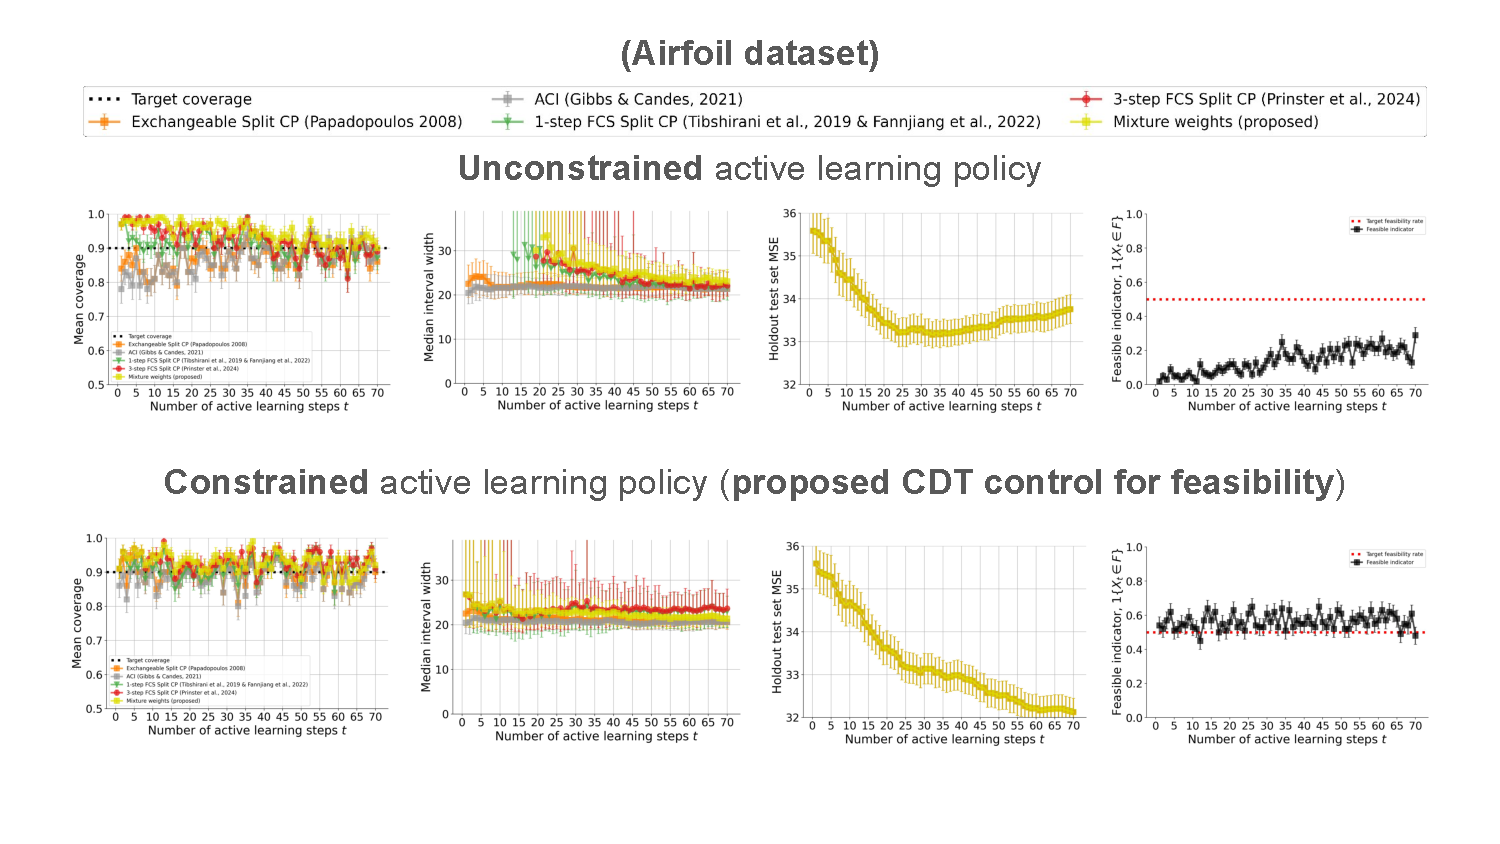
\includegraphics[width=\textwidth]{figures/airfoil.pdf}
    \caption{Results for airfoil UCI dataset.}
\end{figure}

\begin{figure}
    \includegraphics[width=\textwidth]{figures/communities.pdf}
    \caption{Results for communities UCI dataset.}
\end{figure}

\begin{figure}
    \includegraphics[width=\textwidth]{figures/meps.pdf}
    \caption{Results for meps UCI dataset.}
\end{figure}



Experimental details:
\begin{itemize}
    \item \textit{Feasibility labels simulated to decay with 'distance' from source distribution:} Recalling how in our previous paper we simulated selection bias by selecting the training/cal set with probability proportional to $exp(\gamma * X^{pca1})$  where $X^{pca1}$  is the projection of the data onto its 1st principal component, here I sampled feasibility labels from $Bernoulli(p_i)$  where $p_i \propto exp(\gamma * X^{pca1}_i)$ for each point, to simulate the training data being biased toward high feasibility (eg, around 70\%) but the average feasibility across the pool being much lower (eg, around 25\% or so).
    \item \textit{Simplified incumbent policy (for easier implementation here):} Just for simpler implementation at the moment, I just kept the "incumbent policy" as the initial source distribution, meaning that at each t, $\pi_t^{\beta_t} := \beta_t * \pi_0 + (1-\beta_t) * \pi_t^{aggressive}$ , where the difference is using $\pi_0$ in the mixture at the moment rather than $\pi_{t-1}^{\beta_{t-1}}$.
    \item \textit{Addressing "pin" in theory we'd discussed}: Re discussion about "pin" in theory for how much weight to put on the test point when selecting a risk-controlled policy, I changed from using the "expectation" of the weight to using the maximum weight over the pool set. This is more conservative, and I think almost certainly valid, whereas I think there was an issue with how I was thinking about "expected" weight before (where may need to be a weighted average over the weights, to account for how by construction it's much more common to sample points that the policy gives high weight to).
\end{itemize}





\section{Discussion}

\bibliography{references}
\bibliographystyle{icml2025}

\appendix
\section{Appendix}
You may include other additional sections here.



\section{Scratch}


Let $\mathcal{X}$ denote the space of possible inputs/contexts/states (e.g., possible protein sequences $\mathbf{x}\in \mathcal{V}^*$, for a vocabulary $\mathcal{V}$), $\mathcal{Y}$ denote the space of a response/outcome variable we care about (e.g., binding affinity or therapeutic efficacy), and let $a:\mathcal{X}\rightarrow \mathcal{X}$ denote the actions that we can take to modify/change/intervene on the space of states/inputs (e.g., modifying some wild-type seed protein sequence $\mathbf{x_0}$ to some designed sequence $\mathbf{x}'$). Furthermore, at each time $t\in [T]$, let $L_t:=L(a(X_t), Y_t)$ denote some loss/cost to taking action $a(X_t)$ and observing $Y_t$ (e.g., in our running protein design example, it may be necessary to ensure that a designed protein sequence is in some set of \textit{feasible} sequences $\mathcal{F}$, and we could use the loss $L_t(X_t')=\mathbbm{1}\{X_t'\not\in\mathcal{F}\}$). Then, our general decision-making goal is the following:
\begin{align*}
    \argmax_{a_t}\quad u(a_t(X_t)) \quad \text{s.t.} \quad L_t \leq \alpha.
\end{align*}

General proxy problem:
\begin{align*}
    \argmax_{a_t}\quad \mathbb{E}[u(a_t(X_t))] \quad \text{s.t.} \quad \mathbb{E}[L_t] \leq \alpha.
\end{align*}

Proxy problem for protein design example: denote design sequence $X_t':=a_t(X_t)$ and loss $L_t:=\mathbbm{1}\{X_t'\not\in\mathcal{F}\}$:
\begin{align*}
    \argmax_{X_t'}\quad \mathbb{E}[u(X_t')] \quad \text{s.t.} \quad & \mathbb{E}[\mathbbm{1}\{X_t'\not\in\mathcal{F}\}] \leq \alpha \\
    & \mathbb{P}(X_t'\not\in\mathcal{F}) \leq \alpha.
\end{align*}


In particular, assume we start with a pre-trained LLM model $\pi_{\theta_0}(\mathbf{x}):\mathcal{X}\rightarrow [0,1]$ denote a pre-trained model (e.g., LLM) with parameters $\theta_0$, which could be written autoregressively as $\pi_{\theta_0}(\mathbf{x})=\prod_{i=1}^{|\mathbf{x}|}\pi_{\theta_0}(x_i\mid x_{<i})$. Now consider prompting $\pi_{\theta_0}$ with some seed sequence $\mathbf{x}_0$ with the goal of finding some design sequence $\mathbf{x}_0'$ that improves the utility function (e.g., binding affinity: $u(\mathbf{x}_0') - u(\mathbf{x}_0)>\epsilon$. For example, might sample with probabilities 
$$p_{\theta_0}(\mathbf{x}_0'|\mathbf{x}_0)\propto \exp(\beta*(\hat{u}(\mathbf{x}_0') - \hat{u}(\mathbf{x}_0)))$$.

Goal: at each time $t$, propose sequences $X_t'\sim p_{\theta_t}$ s.t. loss is controlled.


% Note that $\pi_{\the`ta_0}$ defines a policy for an initial action, 



the true utility (e.g., binding affinity or therapeutic efficacy) for any sequence $x\in \mathcal{X}$, and $\mathcal{F}\subseteq \mathcal{X}$ the subset of protein sequences that are physically/biologically feasible to produce. The true problem we are interested in is to find a feasible sequence $x'$ that maximizes the utility:
\begin{align}
    x' = \argmax u(x) \quad \text{ s.t. } \quad x \in \mathcal{F}.
\end{align}

In practice, we do not have access to the true utility function $u$, however, so we instead solve a proxy problem. That is, with $\hat{u}:\mathcal{X}\rightarrow \mathbb{R}$ denoting our regression model for the true utility function $u$ and $p(\cdot \mid \hat{u}, D_{1:(t-1)})$ denoting our policy for sampling design sequences (e.g., $p(\cdot \mid \hat{u}, D_{1:(t-1)}) \propto \exp(\beta \cdot \hat{u})$ for some temperature parameter $\beta$), in practice we try to solve
\begin{align}
    x_t = \argmax \mathbb{E}[u(x)] \quad \text{ s.t. }\quad \mathbb{P}(x_t \not\in \mathcal{F})\leq \alpha \quad \forall \quad t.
\end{align}





\textbf{Problem formulation:} There are a few aesthetic choices we should make to determine how to frame our problem, which can all yield equivalent formulations, but affect framing:
\begin{itemize}
    \item \textbf{Objective:} Minimizing loss vs maximizing utility
    \item \textbf{Constraint:} Helpful to decide if constraint is on the objective function directly, or if is on a separate cost function. Additionally, different types of constraints:
    \begin{itemize}
        \item \textit{Controlling risk in expectation} (e.g., \citet{angelopoulos2022conformal}): Want expectation of loss to be below some \textit{user-specified, fixed} $\alpha$:
        \begin{align}
            \mathbb{E}[\mathcal{L}(a(X),Y))] \leq \alpha
        \end{align}\label{eq:risk_control}
        \drew{Note: There may not be an action $a$ that satisfies this.}
        \item \textit{Controlling risk in probability} (e.g., contextual bandits): Want probability of the loss exceeding some \textit{fixed} safety-threshold $\tau$ to be no more than some \textit{user-specified, fixed} $\alpha$:
        \begin{align}
            & \mathbb{P}[l(a(X),Y)) > \tau] \leq \alpha \\
            \iff & \mathbb{E}[\mathbbm{1}\{l(a(X),Y)) > \tau\}] \leq \alpha \nonumber \\
            \iff & \eqref{eq:risk_control} \ \text{ if } \ \mathcal{L}(a(X),Y)) = \mathbbm{1}\{l(a(X),Y)) > \tau\} \nonumber 
        \end{align}
        \drew{Note: There may not be an action $a$ that satisfies this.}
        \item \textit{Risk assessment} (e.g., \citet{prinster2022jaws}): \textit{Find minimum upper-bound}, $\alpha_R$, on the probability that an action is unsafe---i.e., exceeds a user-specified, \textit{fixed safety threshold,} $\tau$:
        \begin{align*}
            \alpha_R = \min\big(\big\{\alpha' \ : \ \mathbb{P}[l(a(X),Y)) > \tau] \leq \alpha'\big\}\big)
        \end{align*}
        \item \textit{Optimizing value-at-risk} (e.g., \citet{kiyani2025decision}): Maximize largest value such that, if action $a$ is taken when facing $x$, then utility is at least $\nu(a;x)$ with probability at least some \textit{user-specified, fixed} $1-\alpha$:
        \begin{align*}
            \max_{a, \nu} \quad & \mathbb{E}_{a, \nu}\big[\nu(X)\big] \nonumber \\
            s.t. \quad \& \mathbb{P}\big[u(a(X),Y)\geq \nu(X)\big] \geq 1-\alpha.
        \end{align*}
        Framed in terms of losses rather than utilities (i.e., letting $l=-u$ and $\tau(\cdot)=-\nu(\cdot)$, this is
        \begin{align*}
            \min_{a, \tau} \quad & \mathbb{E}_{a, \tau}\big[\tau(X)\big] \nonumber \\
            s.t. \quad & \mathbb{P}\big[l(a(X),Y)\geq \tau(X)\big] \leq \alpha.
        \end{align*}
    \end{itemize}
\end{itemize}


Let $\mathcal{X}$ denote the space of potential protein sequences, $u(x):\mathcal{X}\rightarrow \mathbb{R}$ denote the true utility (e.g., binding affinity or therapeutic efficacy) for any sequence $x\in \mathcal{X}$, and $\mathcal{F}\subseteq \mathcal{X}$ the subset of protein sequences that are physically/biologically feasible to produce. The true problem we are interested in is to find a feasible sequence $x'$ that maximizes the utility:
\begin{align}
    x' = \argmax u(x) \quad \text{ s.t. } \quad x \in \mathcal{F}.
\end{align}

In practice, we do not have access to the true utility function $u$, however, so we instead solve a proxy problem. That is, with $\hat{u}:\mathcal{X}\rightarrow \mathbb{R}$ denoting our regression model for the true utility function $u$ and $p(\cdot \mid \hat{u}, D_{1:(t-1)})$ denoting our policy for sampling design sequences (e.g., $p(\cdot \mid \hat{u}, D_{1:(t-1)}) \propto \exp(\beta \cdot \hat{u})$ for some temperature parameter $\beta$), in practice we try to solve
\begin{align}
    x_t = \argmax \mathbb{E}[u(x)] \quad \text{ s.t. }\quad \mathbb{P}(x_t \not\in \mathcal{F})\leq \alpha \quad \forall \quad t.
\end{align}

\drew{Note: Update notation in proxy problem to be more explicit}

\drew{Question: In practice, is only one designed sequence sent to the lab at a time? Or, are several candidates all sent at the same time?}

Potentially could consider stronger versions of the constraint, i.e., sequential anytime-valid version, which would control the probability of \textit{ever} having a proposed design sequence that's not feasible:
\begin{align}
    \mathbb{P}(\exists \  t : \ x_t \not\in \mathcal{F})\leq \alpha
\end{align}
However, the anytime-valid control is often considered overly conservative, as it controls the probability of a false positive \textit{ever} occuring in an infinite sequence. An intermediately-strong constraint could be instead to control the probability of a false positive among a batch of $T$ designed sequences, i.e., an infeasible sequence at some time $t\in [T]:=\{1, ..., T\}$:
\begin{align}
    \mathbb{P}(\exists \  t \in [T] : \ x_t \not\in \mathcal{F})\leq \alpha
\end{align}



\subsection{Initial draft from Sam}

We train a policy $\pi_\theta(x' \mid x)$ using the FReKL loss on a dataset of matched improving pairs constructed as follows. For each pair of sequences $(x, x')$ within a specified edit distance, we assign rewards:
\begin{equation}
r(x, x') = \begin{cases}
\max(f(x') - f(x), 0) & \text{if } x \in \mathcal{F} \text{ and } x' \in \mathcal{F} \\
1 & \text{if } x \notin \mathcal{F} \text{ and } x' \in \mathcal{F} \\
0 & \text{if } x \notin \mathcal{F} \text{ and } x' \notin \mathcal{F} \\
-1 & \text{if } x \in \mathcal{F} \text{ and } x' \notin \mathcal{F}
\end{cases}
\end{equation}
where $\mathcal{F}$ denotes the feasible set and $f$ is the objective function. This reward structure encourages the policy to maintain feasibility while seeking improvements, with explicit penalties for constraint violations.

To generate queries with controlled risk, we sample a library $\mathcal{L} = \{(x_i, x'_i)\}_{i=1}^N$ from the trained policy and define a nonconformity score $s(x, x') = -\log \pi_\theta(x' \mid x)$.
\textcolor{red}{Consider $-\log \pi_\theta(x' \mid x) - \log \hat p(x)$, where $\hat p(x)$ is our estimate of the prompt distribution.}
We seek a threshold $\beta$ such that the filtered set
\begin{equation}
\mathcal{C}_\beta = \{(x, x') \in \mathcal{L} : s(x, x') \leq \beta\}
\end{equation}
satisfies the risk constraint $\mathbb{E}[\mathbf{1}\{x' \notin \mathcal{F}\}] \leq \alpha$ for a user-specified tolerance $\alpha$.

\drew{Conformal risk control requires that the loss function, in this case $L_i(\beta):=\mathbbm{1}\{x_j'\not\in\mathcal{F}\}$, is \textit{non-increasing} in $\beta$. In what's written here, however, increasing $\beta$ seems like it would \textit{increase} $L_i(\beta):=\mathbbm{1}\{x_j'\not\in\mathcal{F}\}$; in other words, increasing the size of the filtered set seems like it would \textit{increase} the rate at which the designed sequence is infeasible... It might work, however, if instead use the threshold as $1/\beta$ in the above.}

Since our calibration data $\mathcal{D}_{\text{cal}} = \{(x_j, x'_j, \mathbf{1}\{x'_j \in \mathcal{F}\})\}_{j=1}^n$ comes from previous rounds of policy execution, we must account for multi-step feedback covariate shift (MFCS). Let $\pi_t$ denote the policy at round $t$ and $P_t$ the induced data distribution. For calibration data from round $t$ evaluated under the current policy $\pi_T$, we compute importance weights:
\begin{equation}
w_j = \frac{p_T(x_j)}{p_t(x_j)} \approx \frac{\pi_T(x_j)}{\pi_t(x_j)}
\end{equation}
The threshold $\beta$ is then chosen as the smallest value satisfying:
\begin{equation}
\sum_{j=1}^n w_j \mathbf{1}\{s(x_j, x'_j) > \beta\} \mathbf{1}\{x'_j \notin \mathcal{F}\} + \frac{1}{n_{\text{eff}} + 1} \leq \alpha
\end{equation}
where $n_{\text{eff}} = 1/\sum_{j=1}^n w_j^2$ is the effective sample size.

Given the filtered library $\mathcal{C}_\beta$, we construct query batches by sampling uniformly at random without replacement, ensuring each selected transition satisfies the calibrated risk bound while maintaining diversity in exploration.

\vspace{2in}



\end{document}
